% testSetup.tex

\subsection{Robot setup}

The base of PR37 robot is horizontally attached to a vertical pole. At its initial position (also defined as Pose11 in pre-defined robot configurations), the robot is fully extended and the torque load at each actuator sensor is ideally zero. The user should reset joint torque sensor if the data from torque sensor is needed.

\begin{figure}
	\begin{center}
				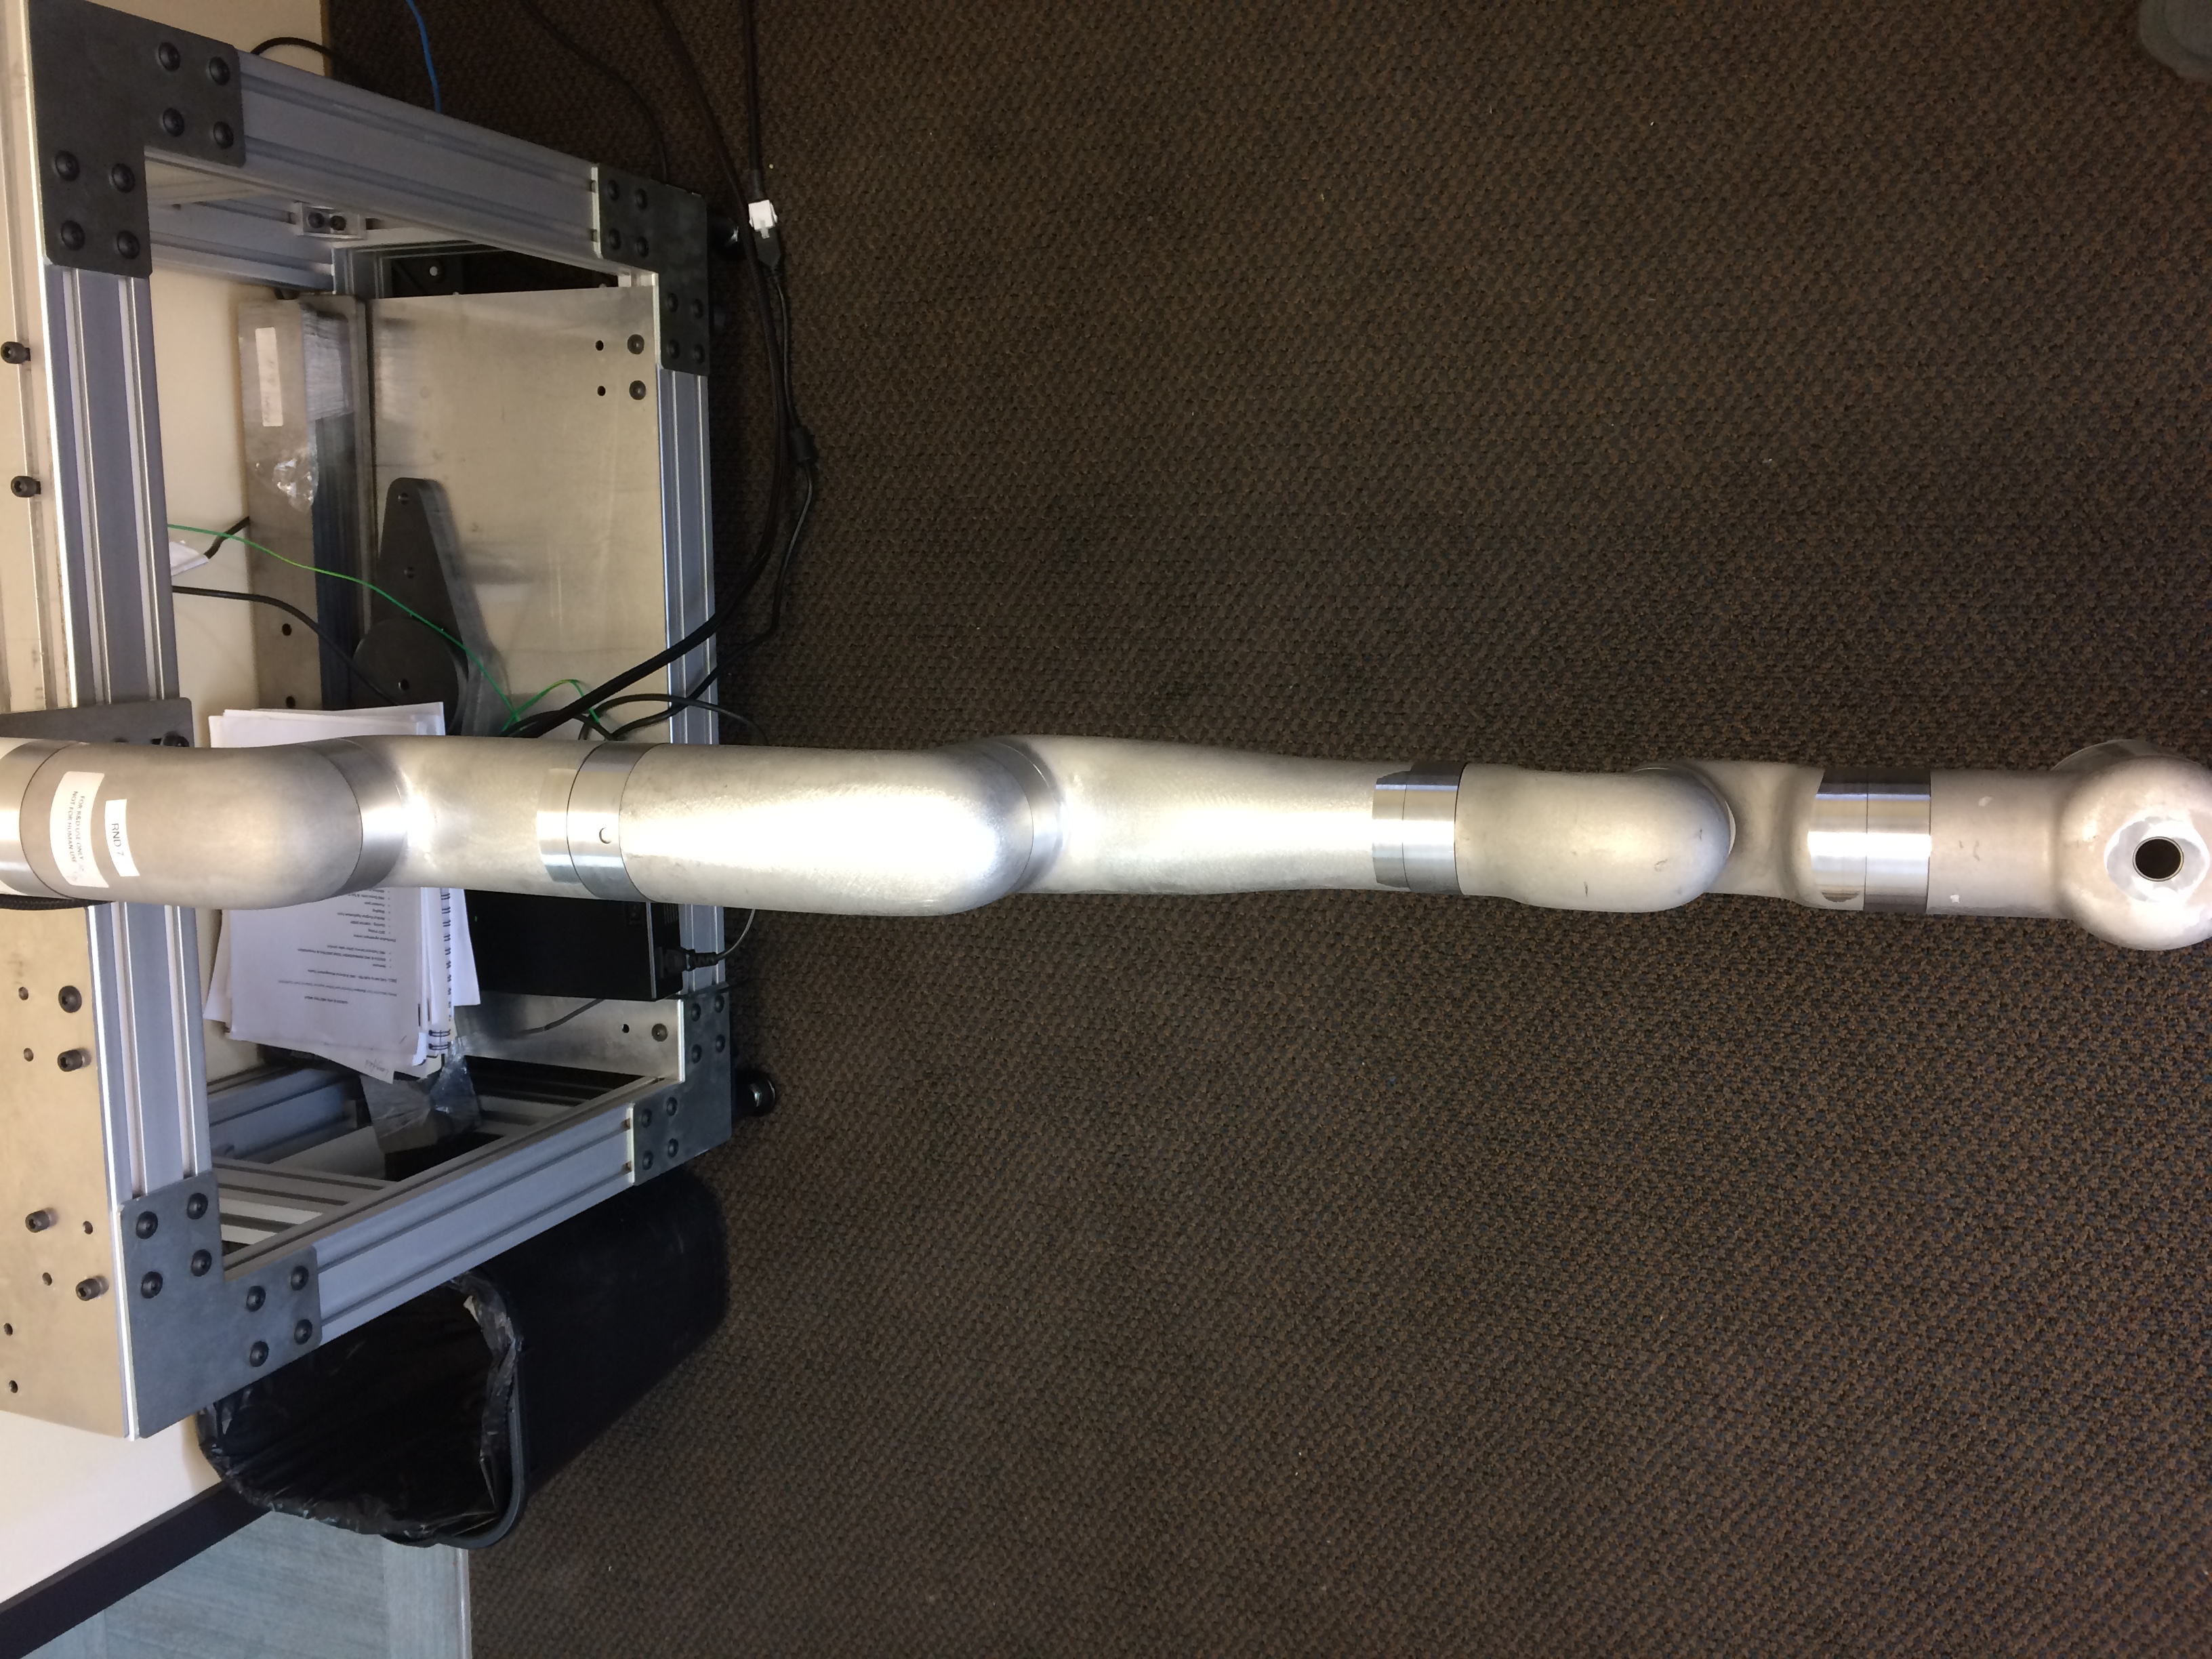
\includegraphics[width=0.9\textwidth]{./images/Pose11}%
		\caption{Test setup}
		\label{fig:pose11}%
	\end{center}
\end{figure}


\subsection{Pre-defined robot configurations}

At each pre-defined robot configuration, the sensor data will be recorded and compared with the gravity model output. Their difference will be used to evaluate the gravity model performance.  At different robot configurations, the torque at each actuator may vary widely. Therefore, the choice of robot configuration for gravity model evaluation is important. 
The pre-defined robot configurations used in this report can be categorized into two groups. 

\textbf{Group A}
In the first group (see in Table \ref{table-groupA}), the robot configurations are provided by Auris from some real user cases. The robot is in a normal operating condition, and these statuses present most common cases. In Pose3, the position command for joint 6 should be 307.70. However, this value provided by Auris cannot be achieved, due to physical limit. In the test, command 307 degree is given in stead. The test and computation regarding to Pose3 are subjected to this minor modification.

\begin{table}[]
	\centering
	\caption{Pre-defined Robot Configuration of Group A (Degrees)}
	\label{table-groupA}
	\begin{tabular}{|l|r|r|r|r|r|r|r|}
		\hline
		\textbf{} & \textbf{Joint1} & \textbf{Joint2} & \textbf{Joint3} & \textbf{Joint4} & \textbf{Joint5} & \textbf{Joint6} & \textbf{Joint7} \\ \hline
		\textbf{Pose 1}  & 115     & 236.85     & 138.2     & 264.09     & 63      & 235.28      & 155.28      \\ \hline
		\textbf{Pose 2}  & 140     & 245.42     & 90.92     & 281.41     & 353.62      & 295.06      & 265.4      \\ \hline
		\textbf{Pose 3}  & 293     & 137.05     & 220.52     & 87.4     & 217.98      & 307      & 103.13      \\ \hline
		\textbf{Pose 4}  & 10     & 176.73     & 147.59     & 43.32     & 142.68      & 275      & 205.12      \\ \hline
		\textbf{Pose 5}  & 85     & 255.93     & 141.29     & 236.09     & 65.84      & 228.26      & 130.5      \\ \hline
		\textbf{Pose 6}  & 140     & 205.51     & 96.12     & 275.16     & 313.2      & 260.62      & 229.57      \\ \hline
		\textbf{Pose 7}  & 120     & 240.31     & 140.2     & 239.88     & 66.74      & 239.24      & 115.38      \\ \hline
		\textbf{Pose 8}  & 285     & 113.25     & 129.73     & 289.67     & 7.89      & 195.54      & 83.44      \\ \hline
		\textbf{Pose 9}  & 285     & 121.22     & 234.46     & 131.94     & 356.65      & 77.01      & 227.27      \\ \hline
		\textbf{Pose 10} & 340    & 141.74    & 22.27    & 67.95    & 16.12     & 61.73     & 153.11      \\ \hline
	\end{tabular}

\end{table}

\begin{figure}
	\centering
	\begin{minipage}{.5\textwidth}
		\centering
		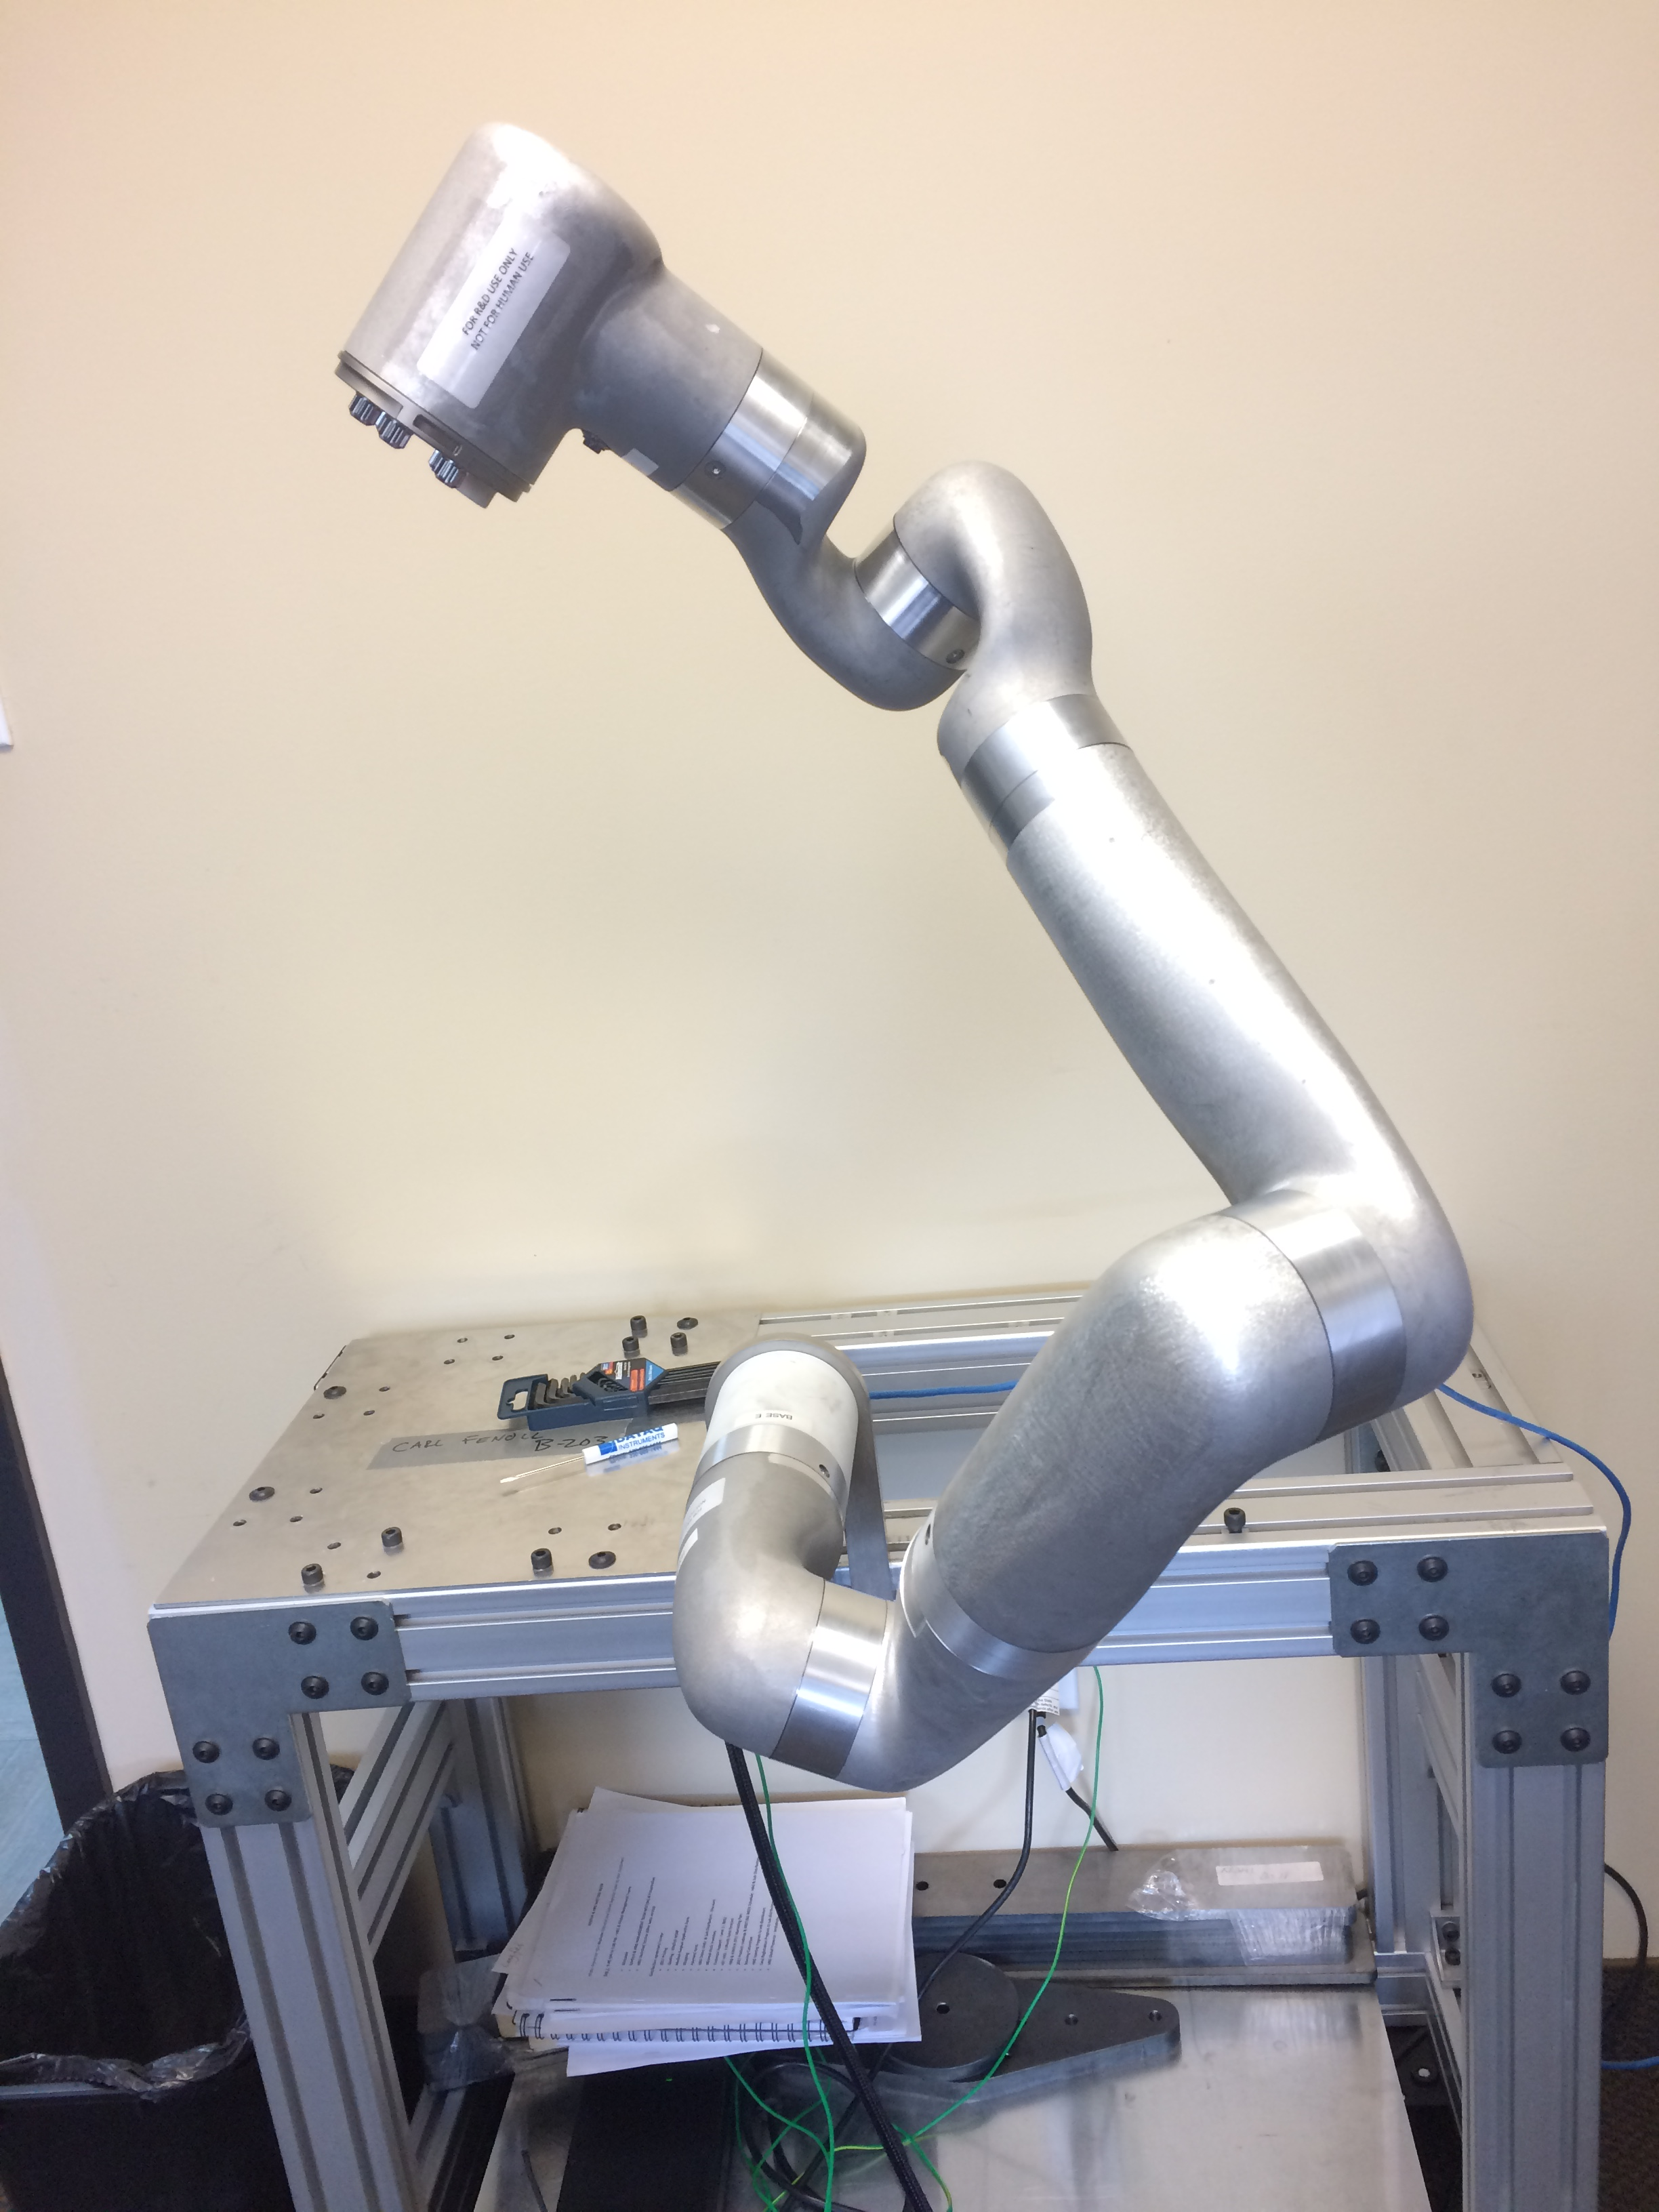
\includegraphics[width=0.9\textwidth]{./images/Pose1}
		\captionof{figure}{Pose1}
		\label{fig:pose1}
	\end{minipage}%
	\begin{minipage}{.5\textwidth}
		\centering
		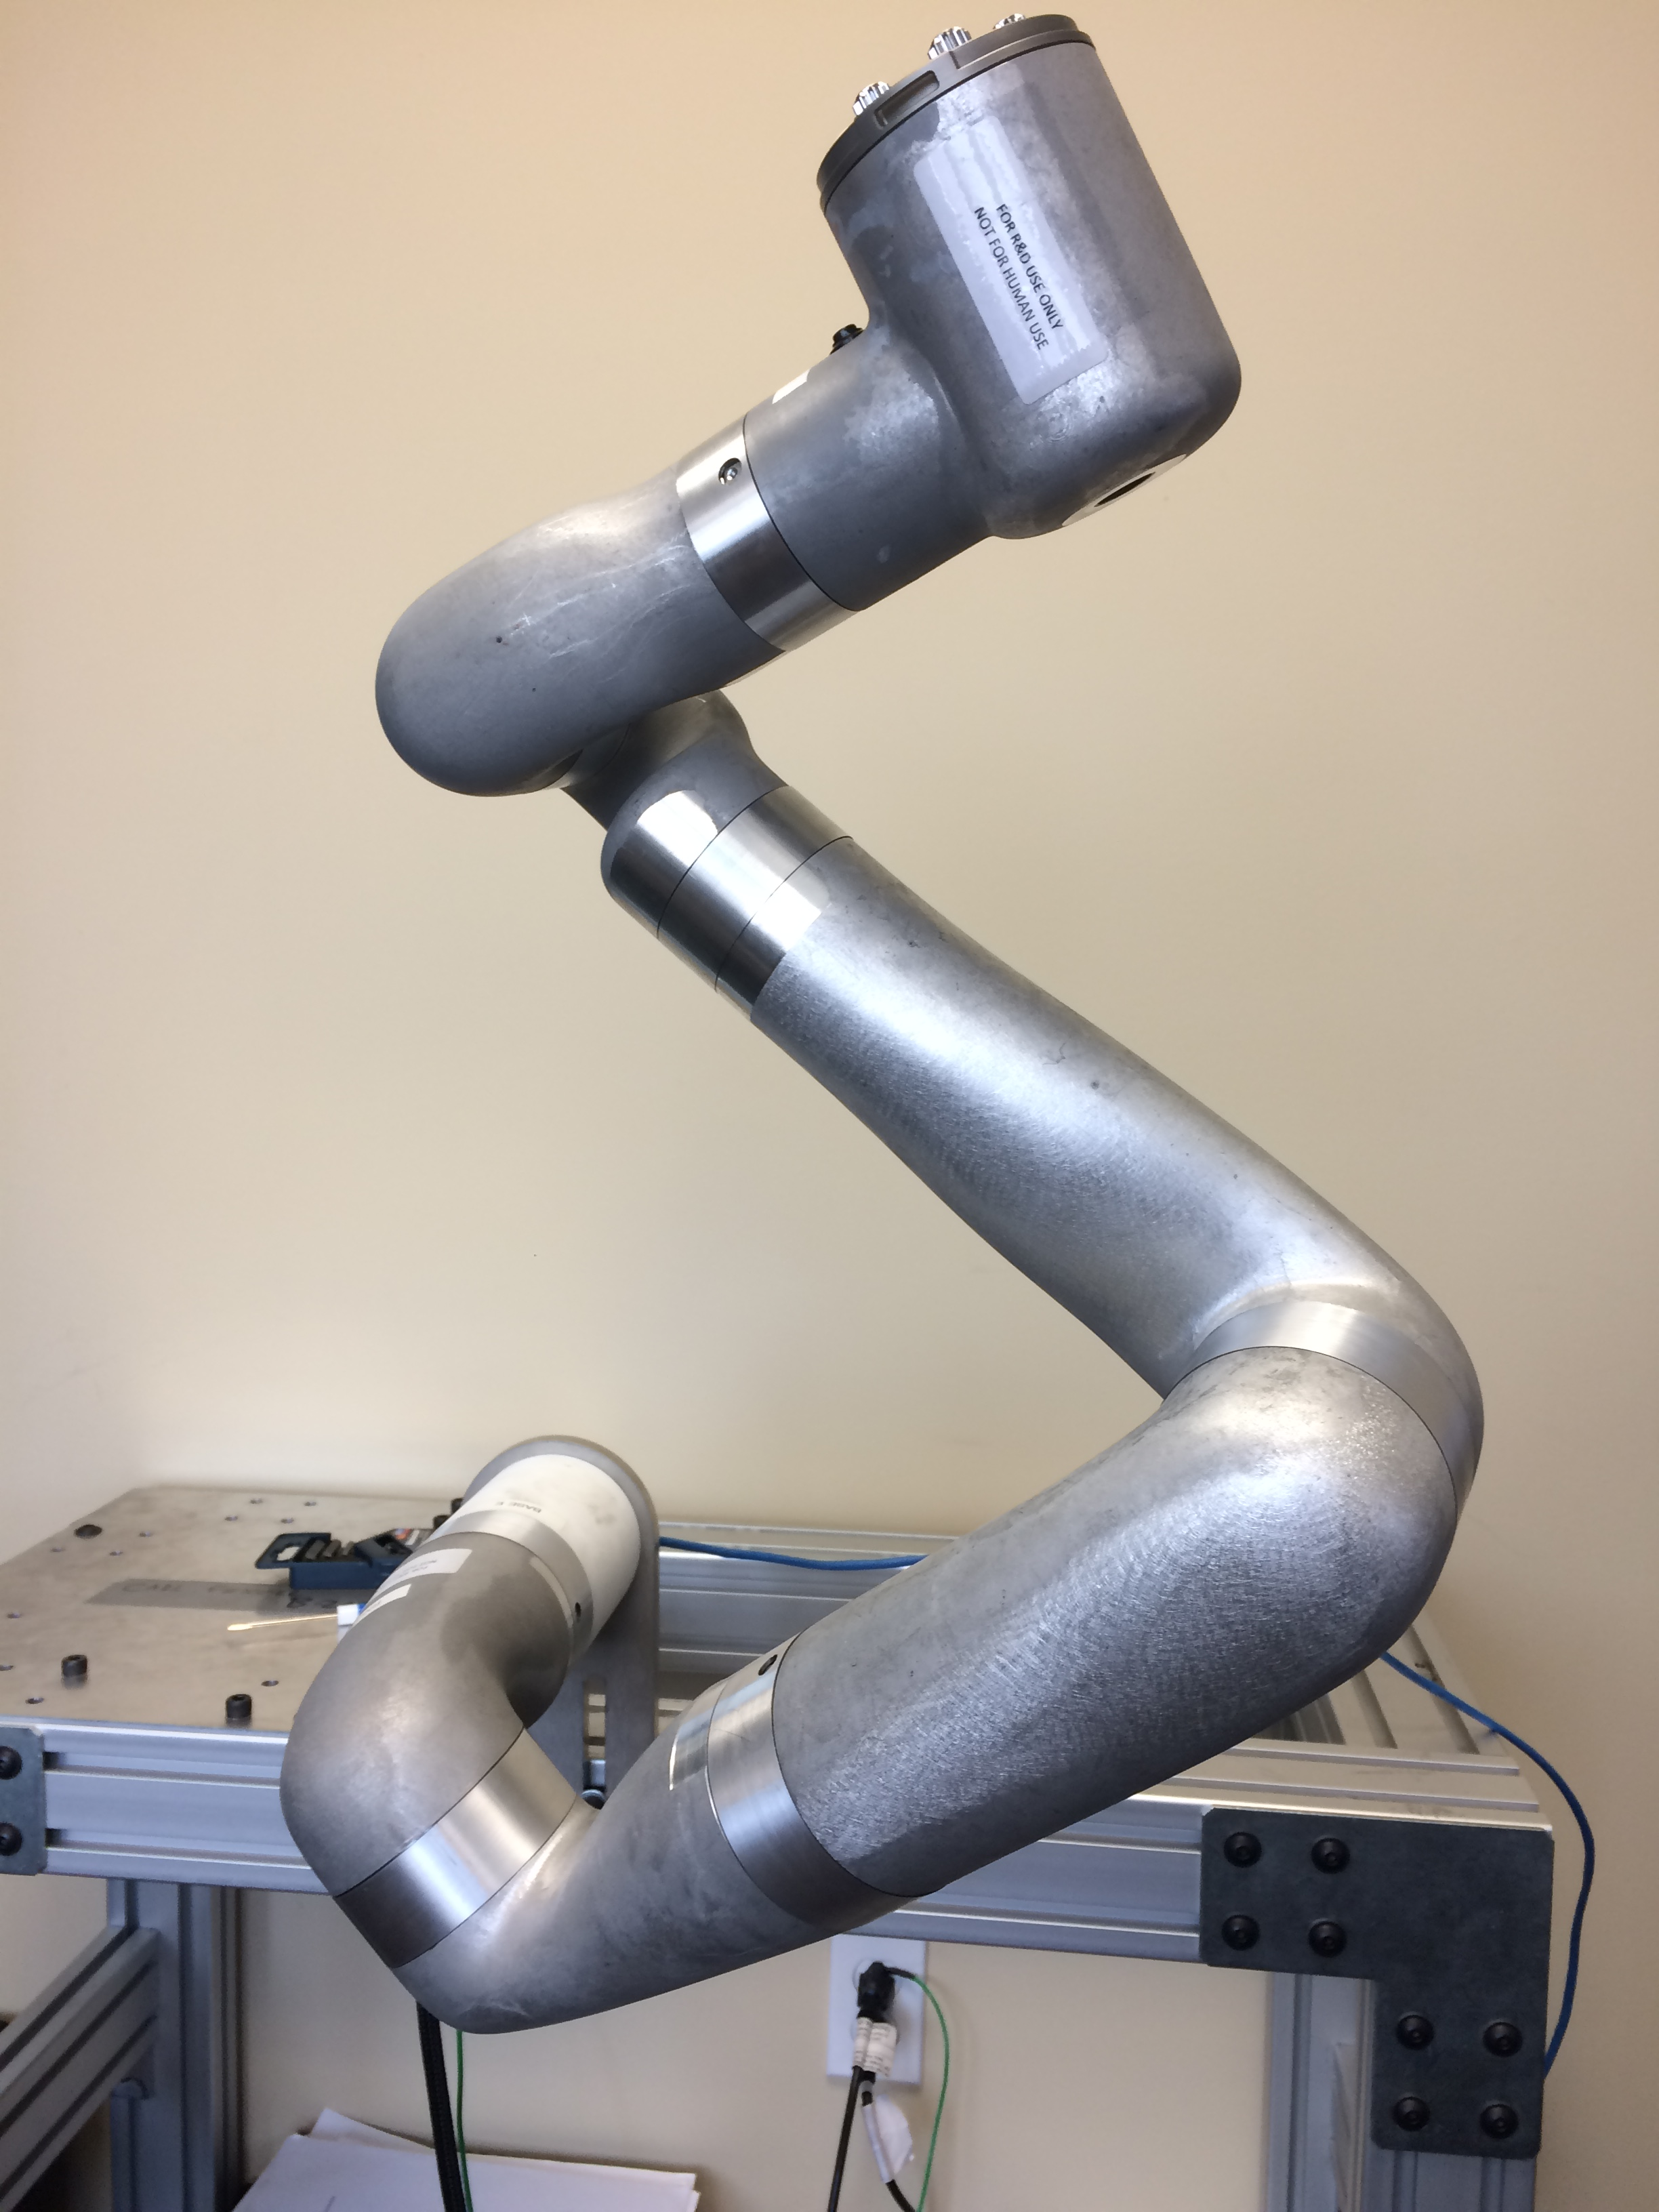
\includegraphics[width=0.9\textwidth]{./images/Pose2}
		\captionof{figure}{Pose2}
		\label{fig:pose2}
	\end{minipage}
\end{figure}

\begin{figure}
	\centering
	\begin{minipage}{.5\textwidth}
		\centering
		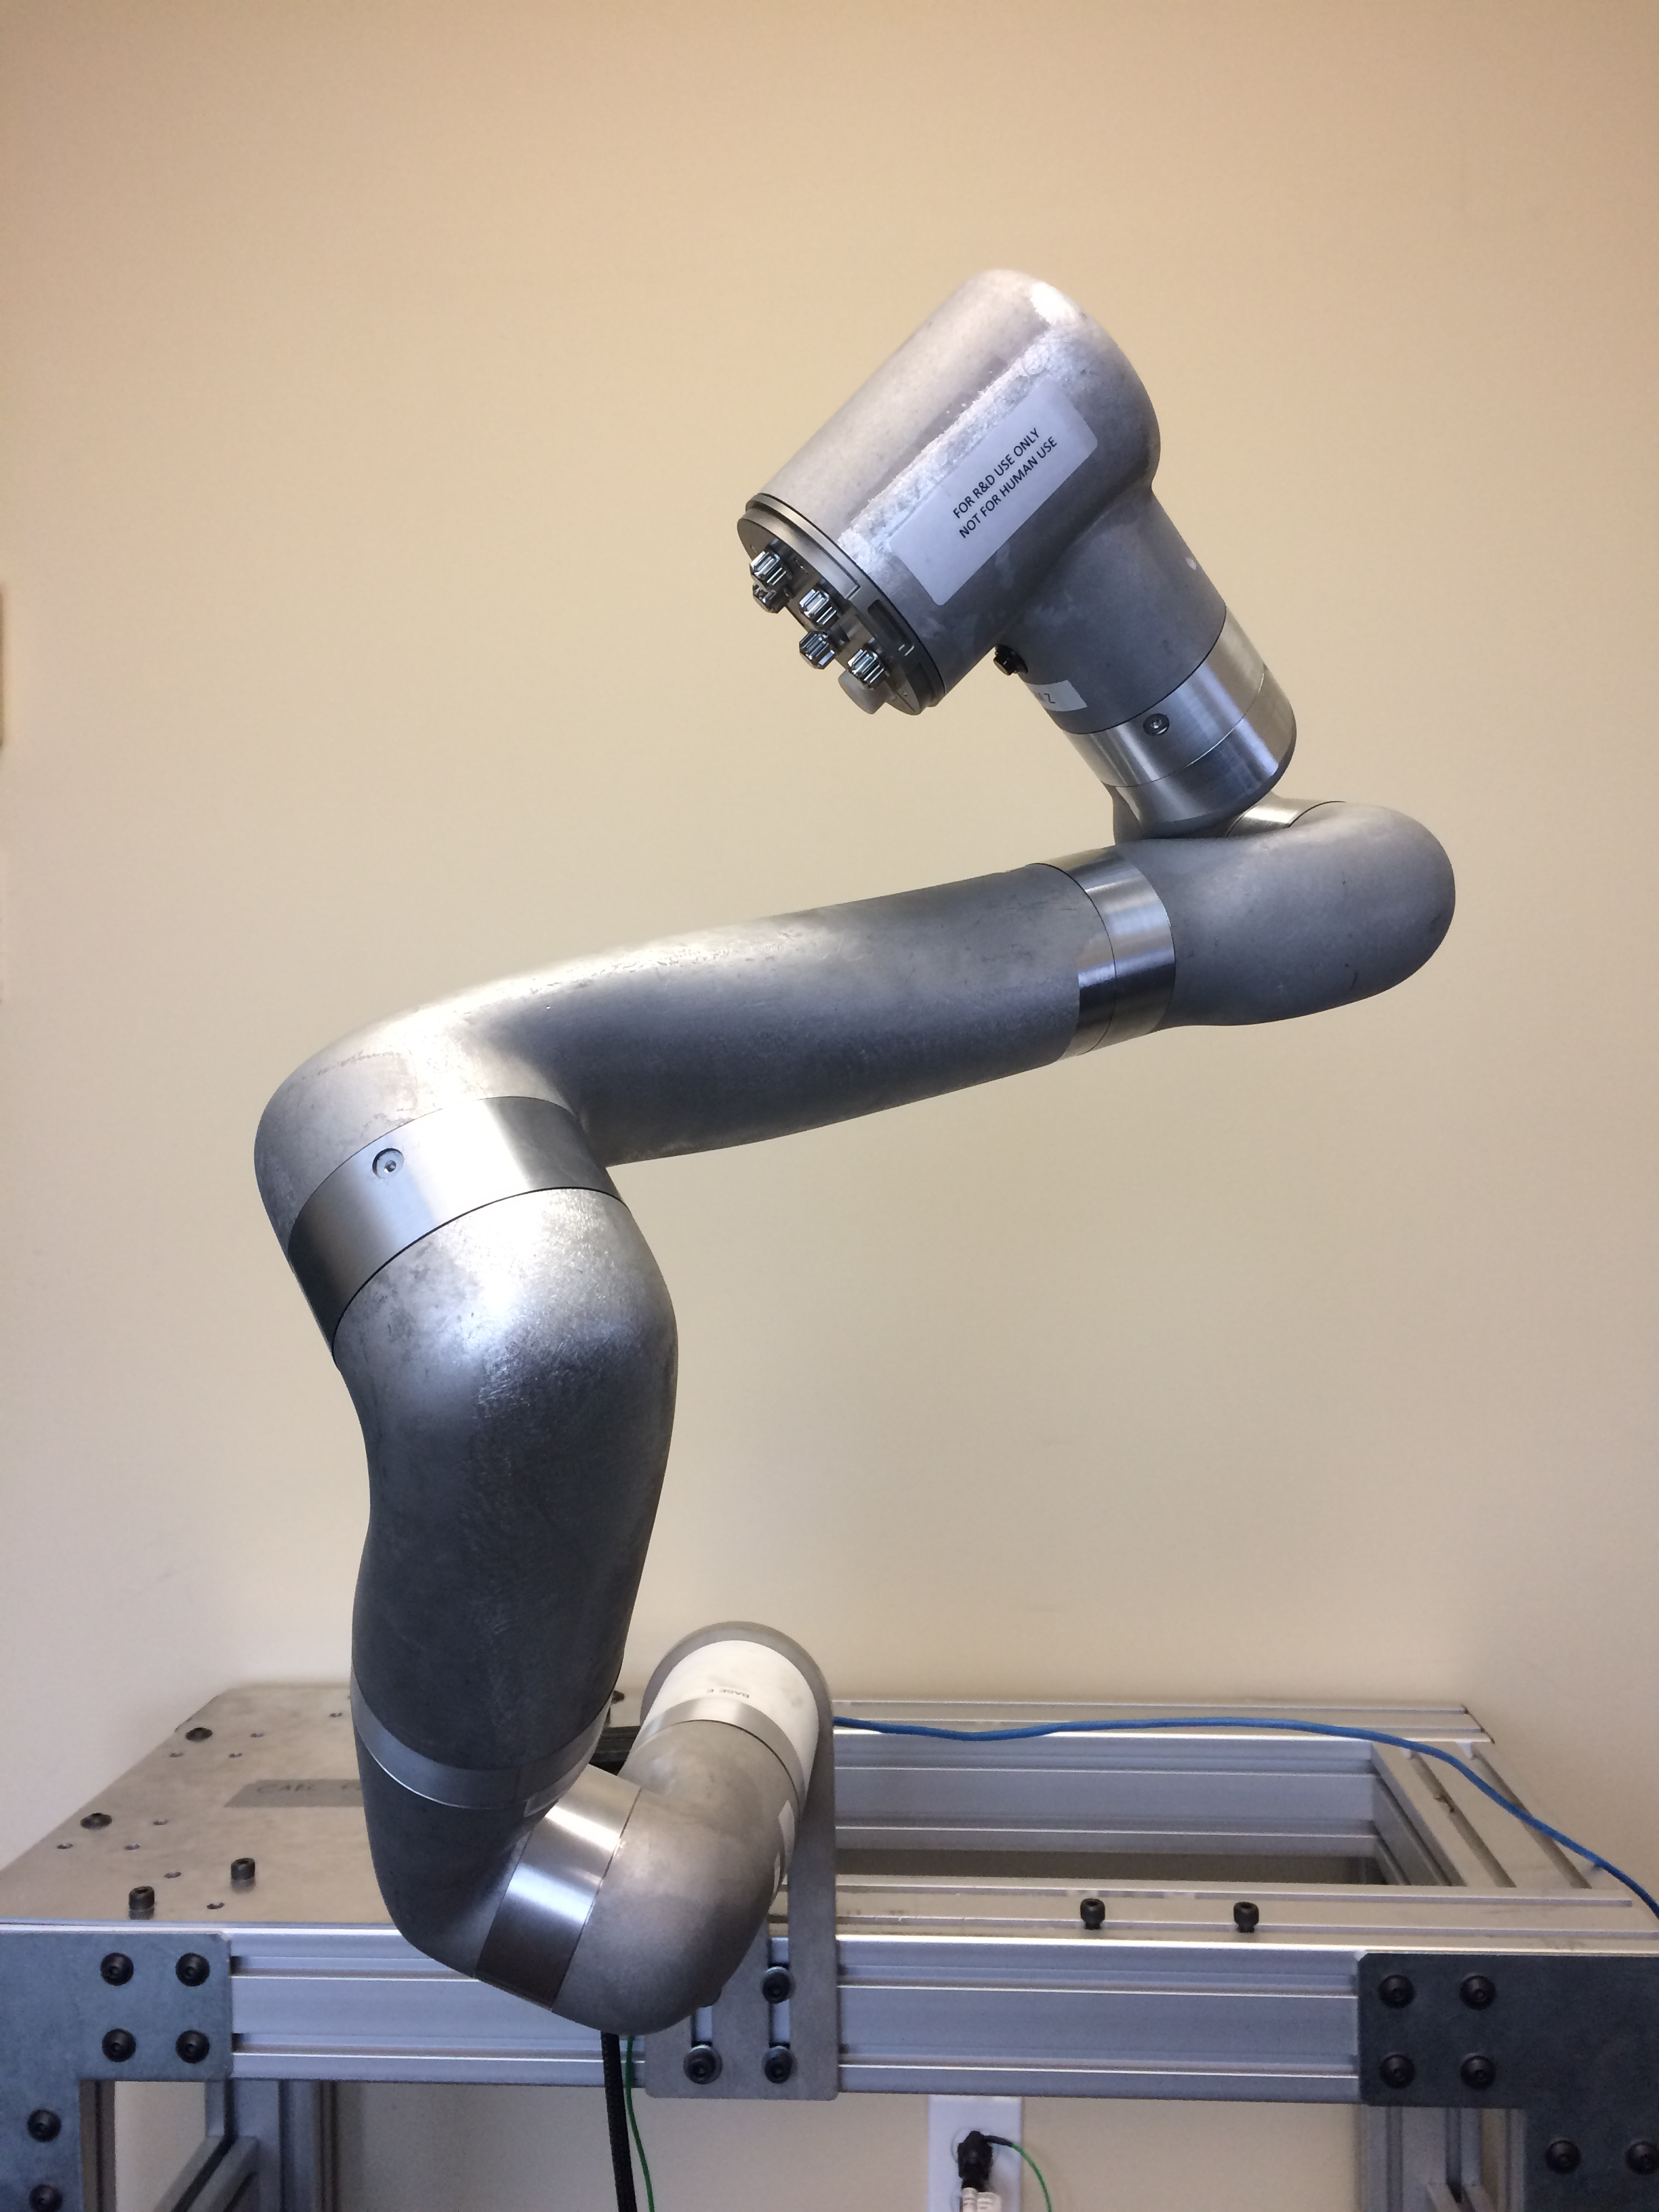
\includegraphics[width=0.9\textwidth]{./images/Pose3}
		\captionof{figure}{Pose3}
		\label{fig:pose3}
	\end{minipage}%
	\begin{minipage}{.5\textwidth}
		\centering
		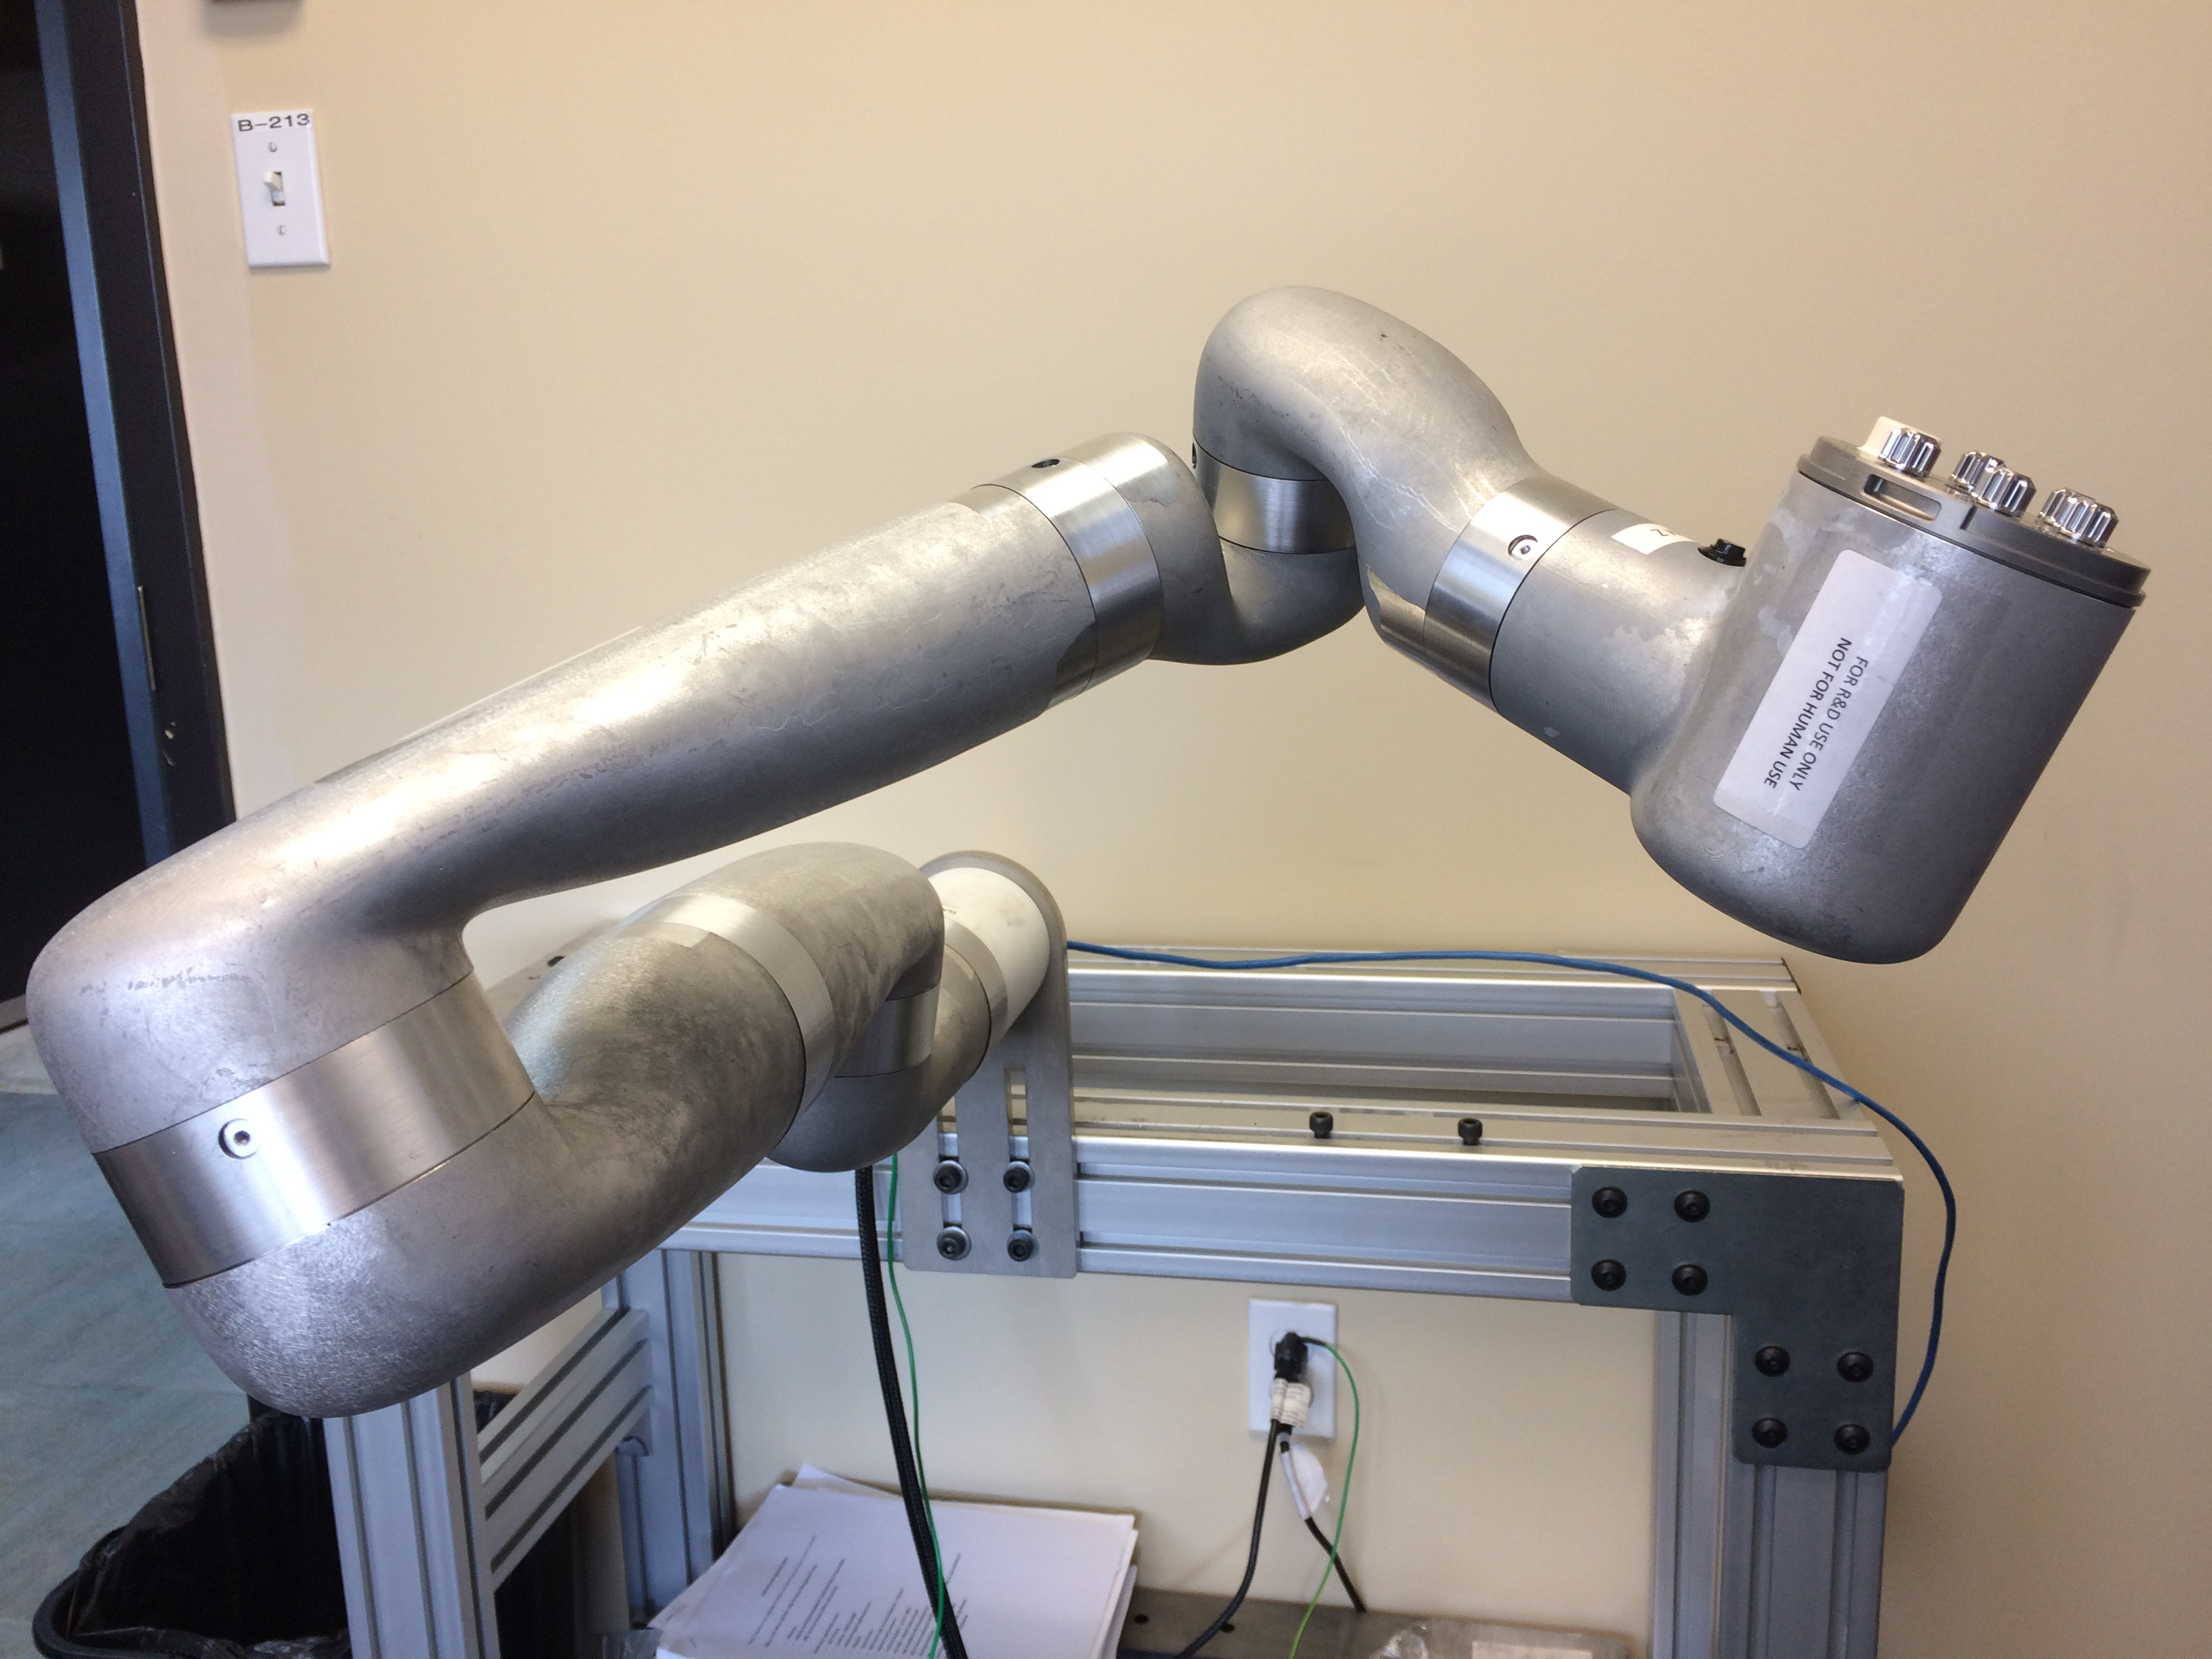
\includegraphics[width=0.9\textwidth]{./images/Pose4}
		\captionof{figure}{Pose4}
		\label{fig:pose4}
	\end{minipage}
\end{figure}

\begin{figure}
	\centering
	\begin{minipage}{.5\textwidth}
		\centering
		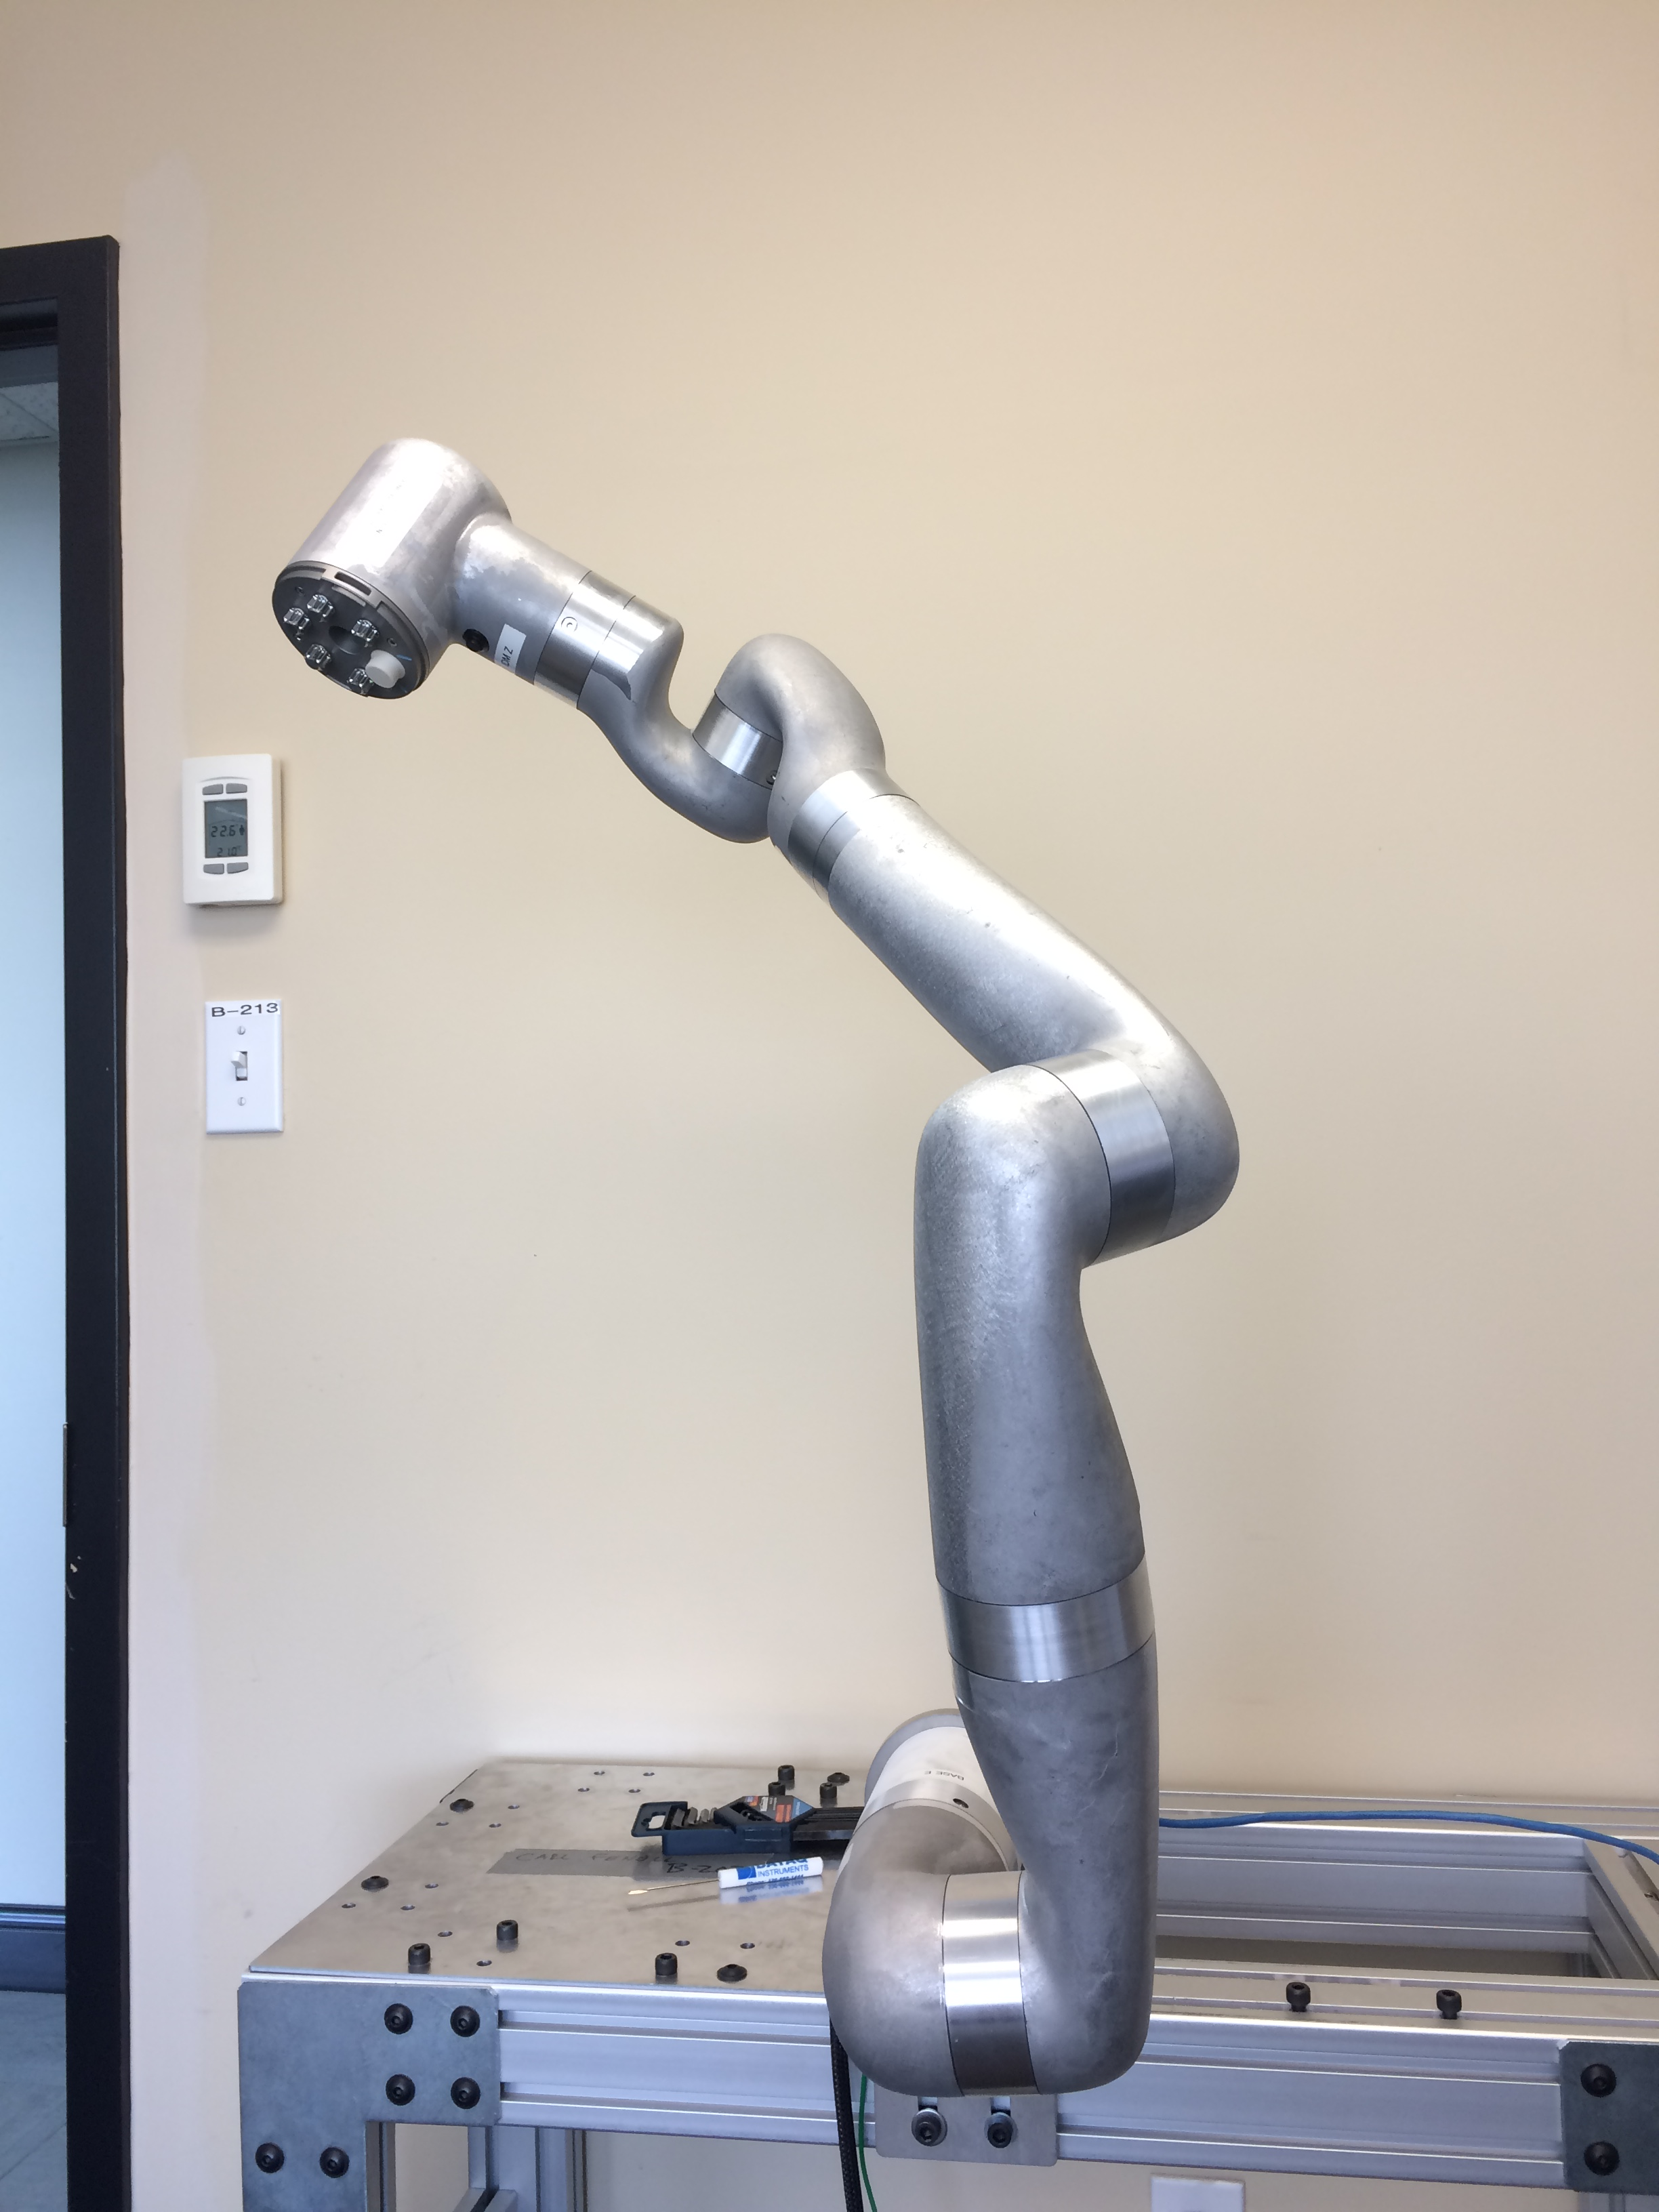
\includegraphics[width=0.9\textwidth]{./images/Pose5}
		\captionof{figure}{Pose5}
		\label{fig:pose5}
	\end{minipage}%
	\begin{minipage}{.5\textwidth}
		\centering
		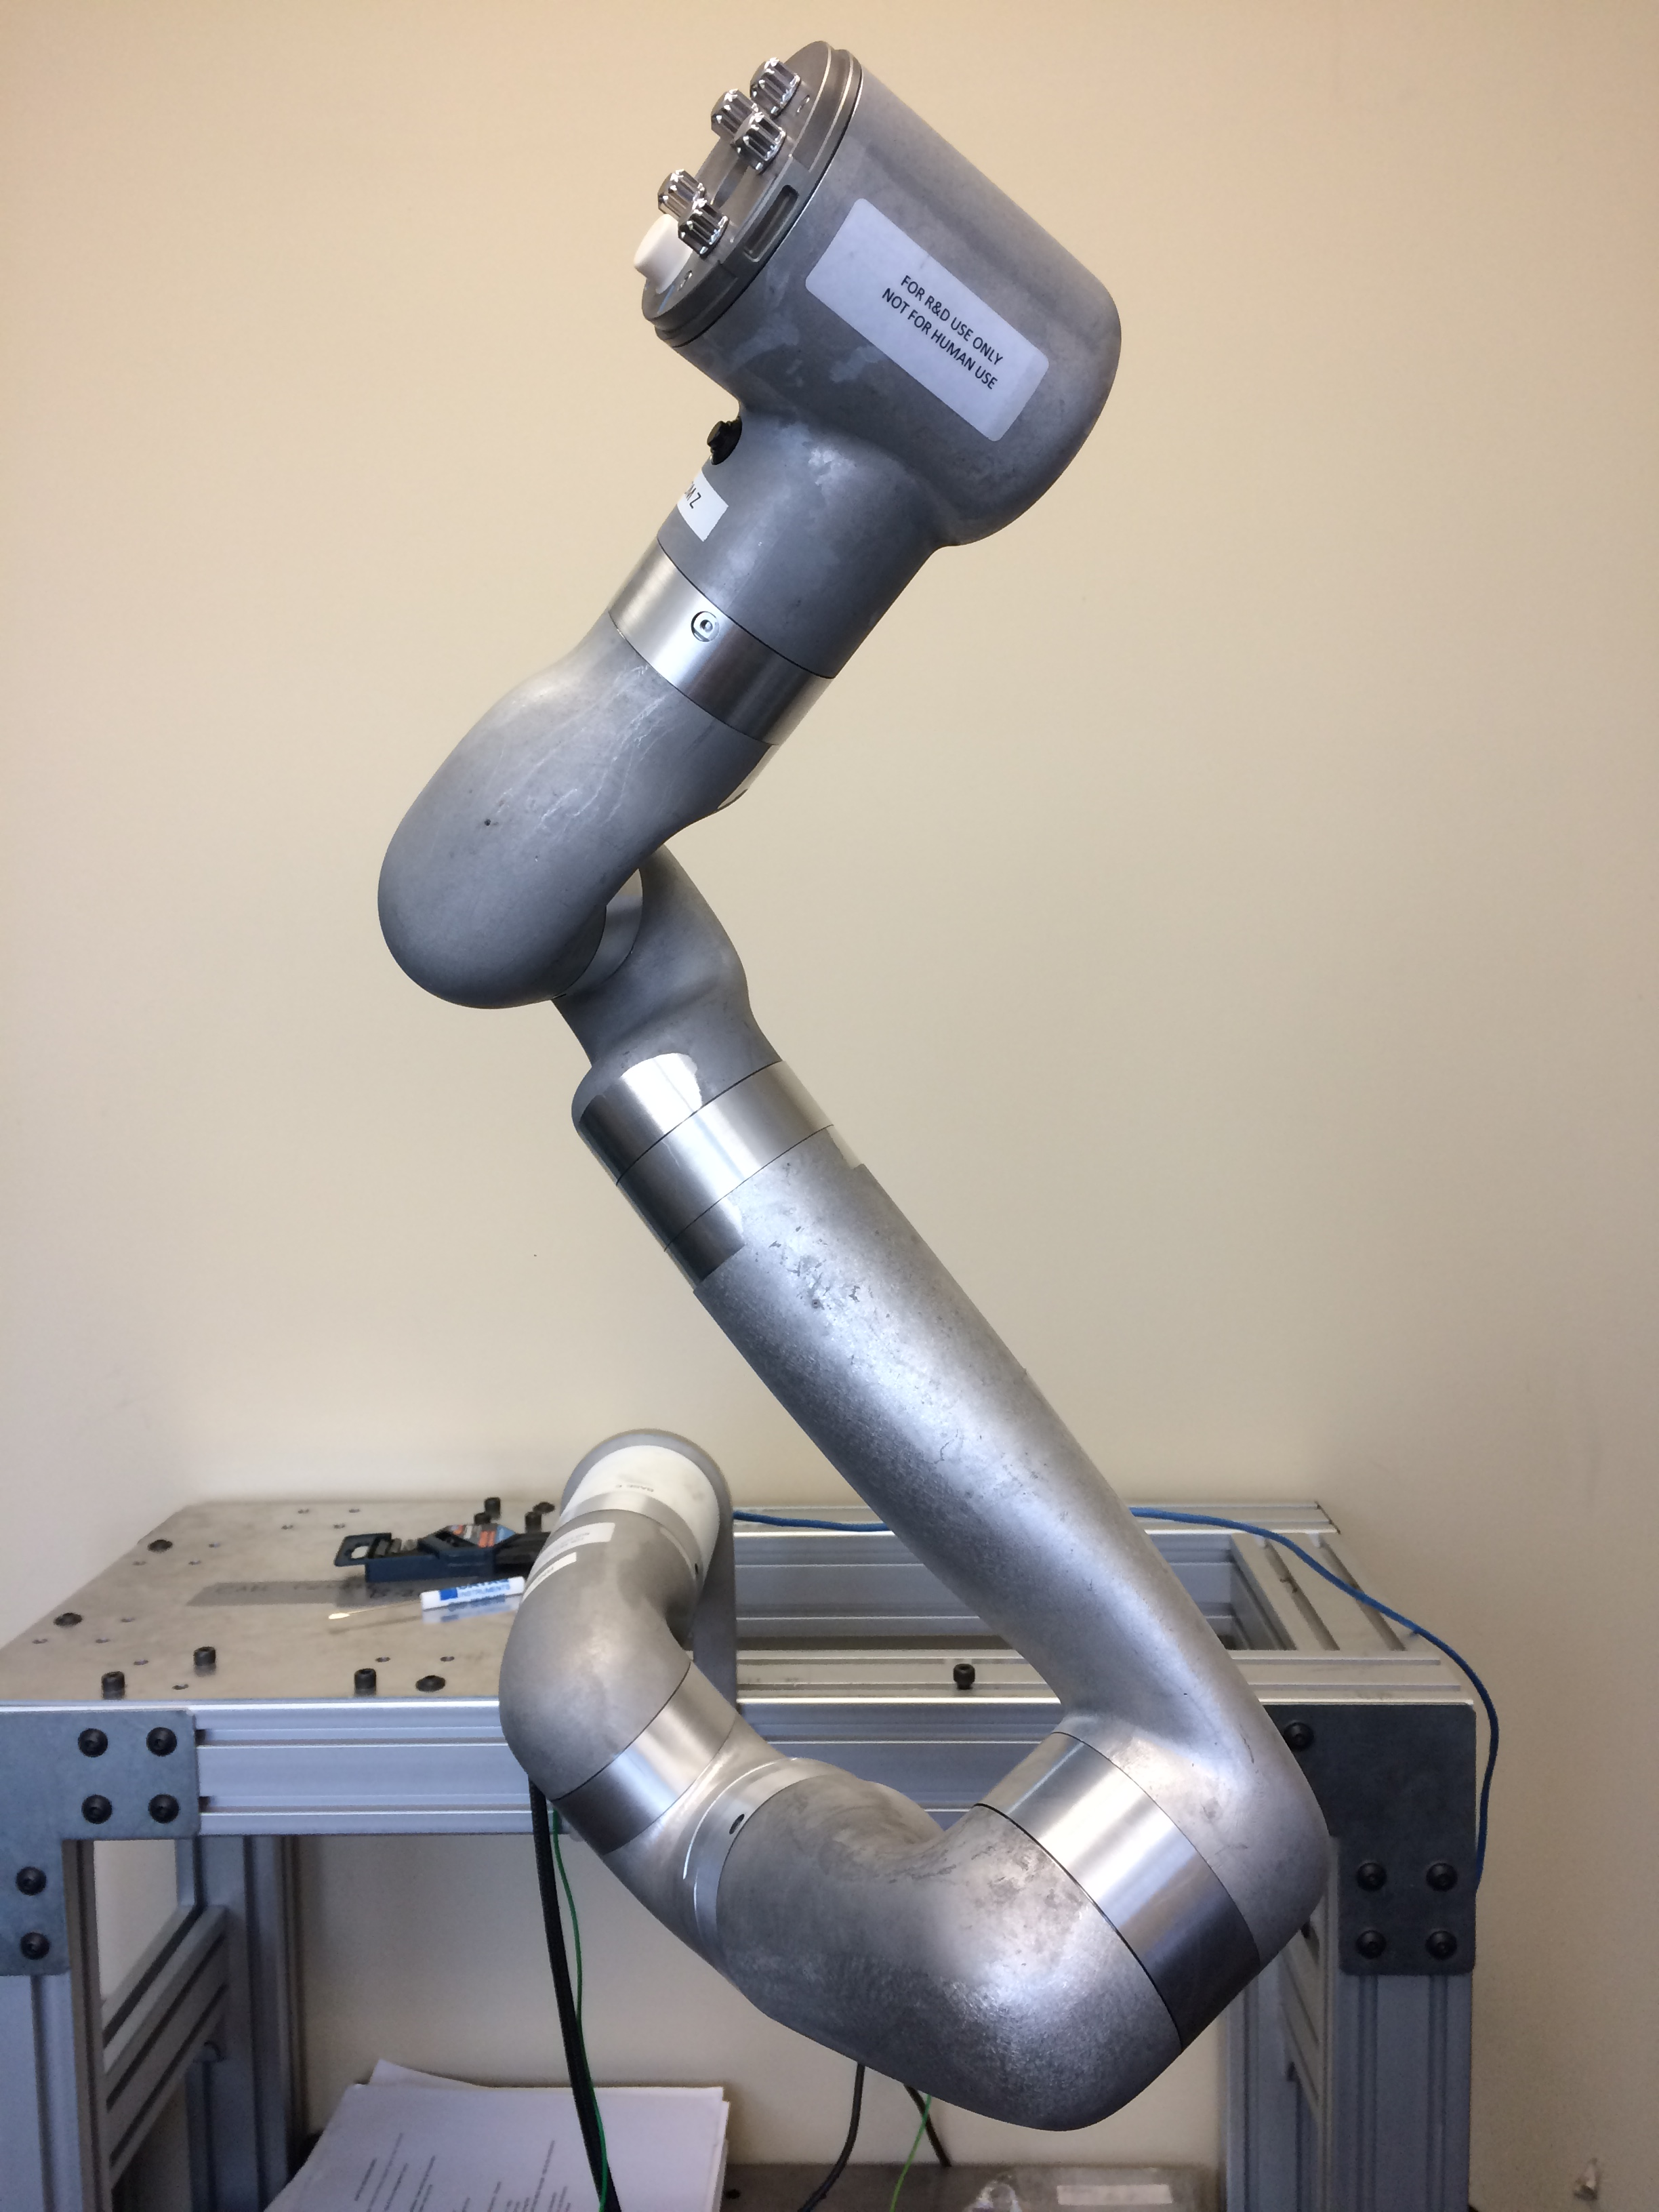
\includegraphics[width=0.9\textwidth]{./images/Pose6}
		\captionof{figure}{Pose6}
		\label{fig:pose6}
	\end{minipage}
\end{figure}

\begin{figure}
	\centering
	\begin{minipage}{.5\textwidth}
		\centering
		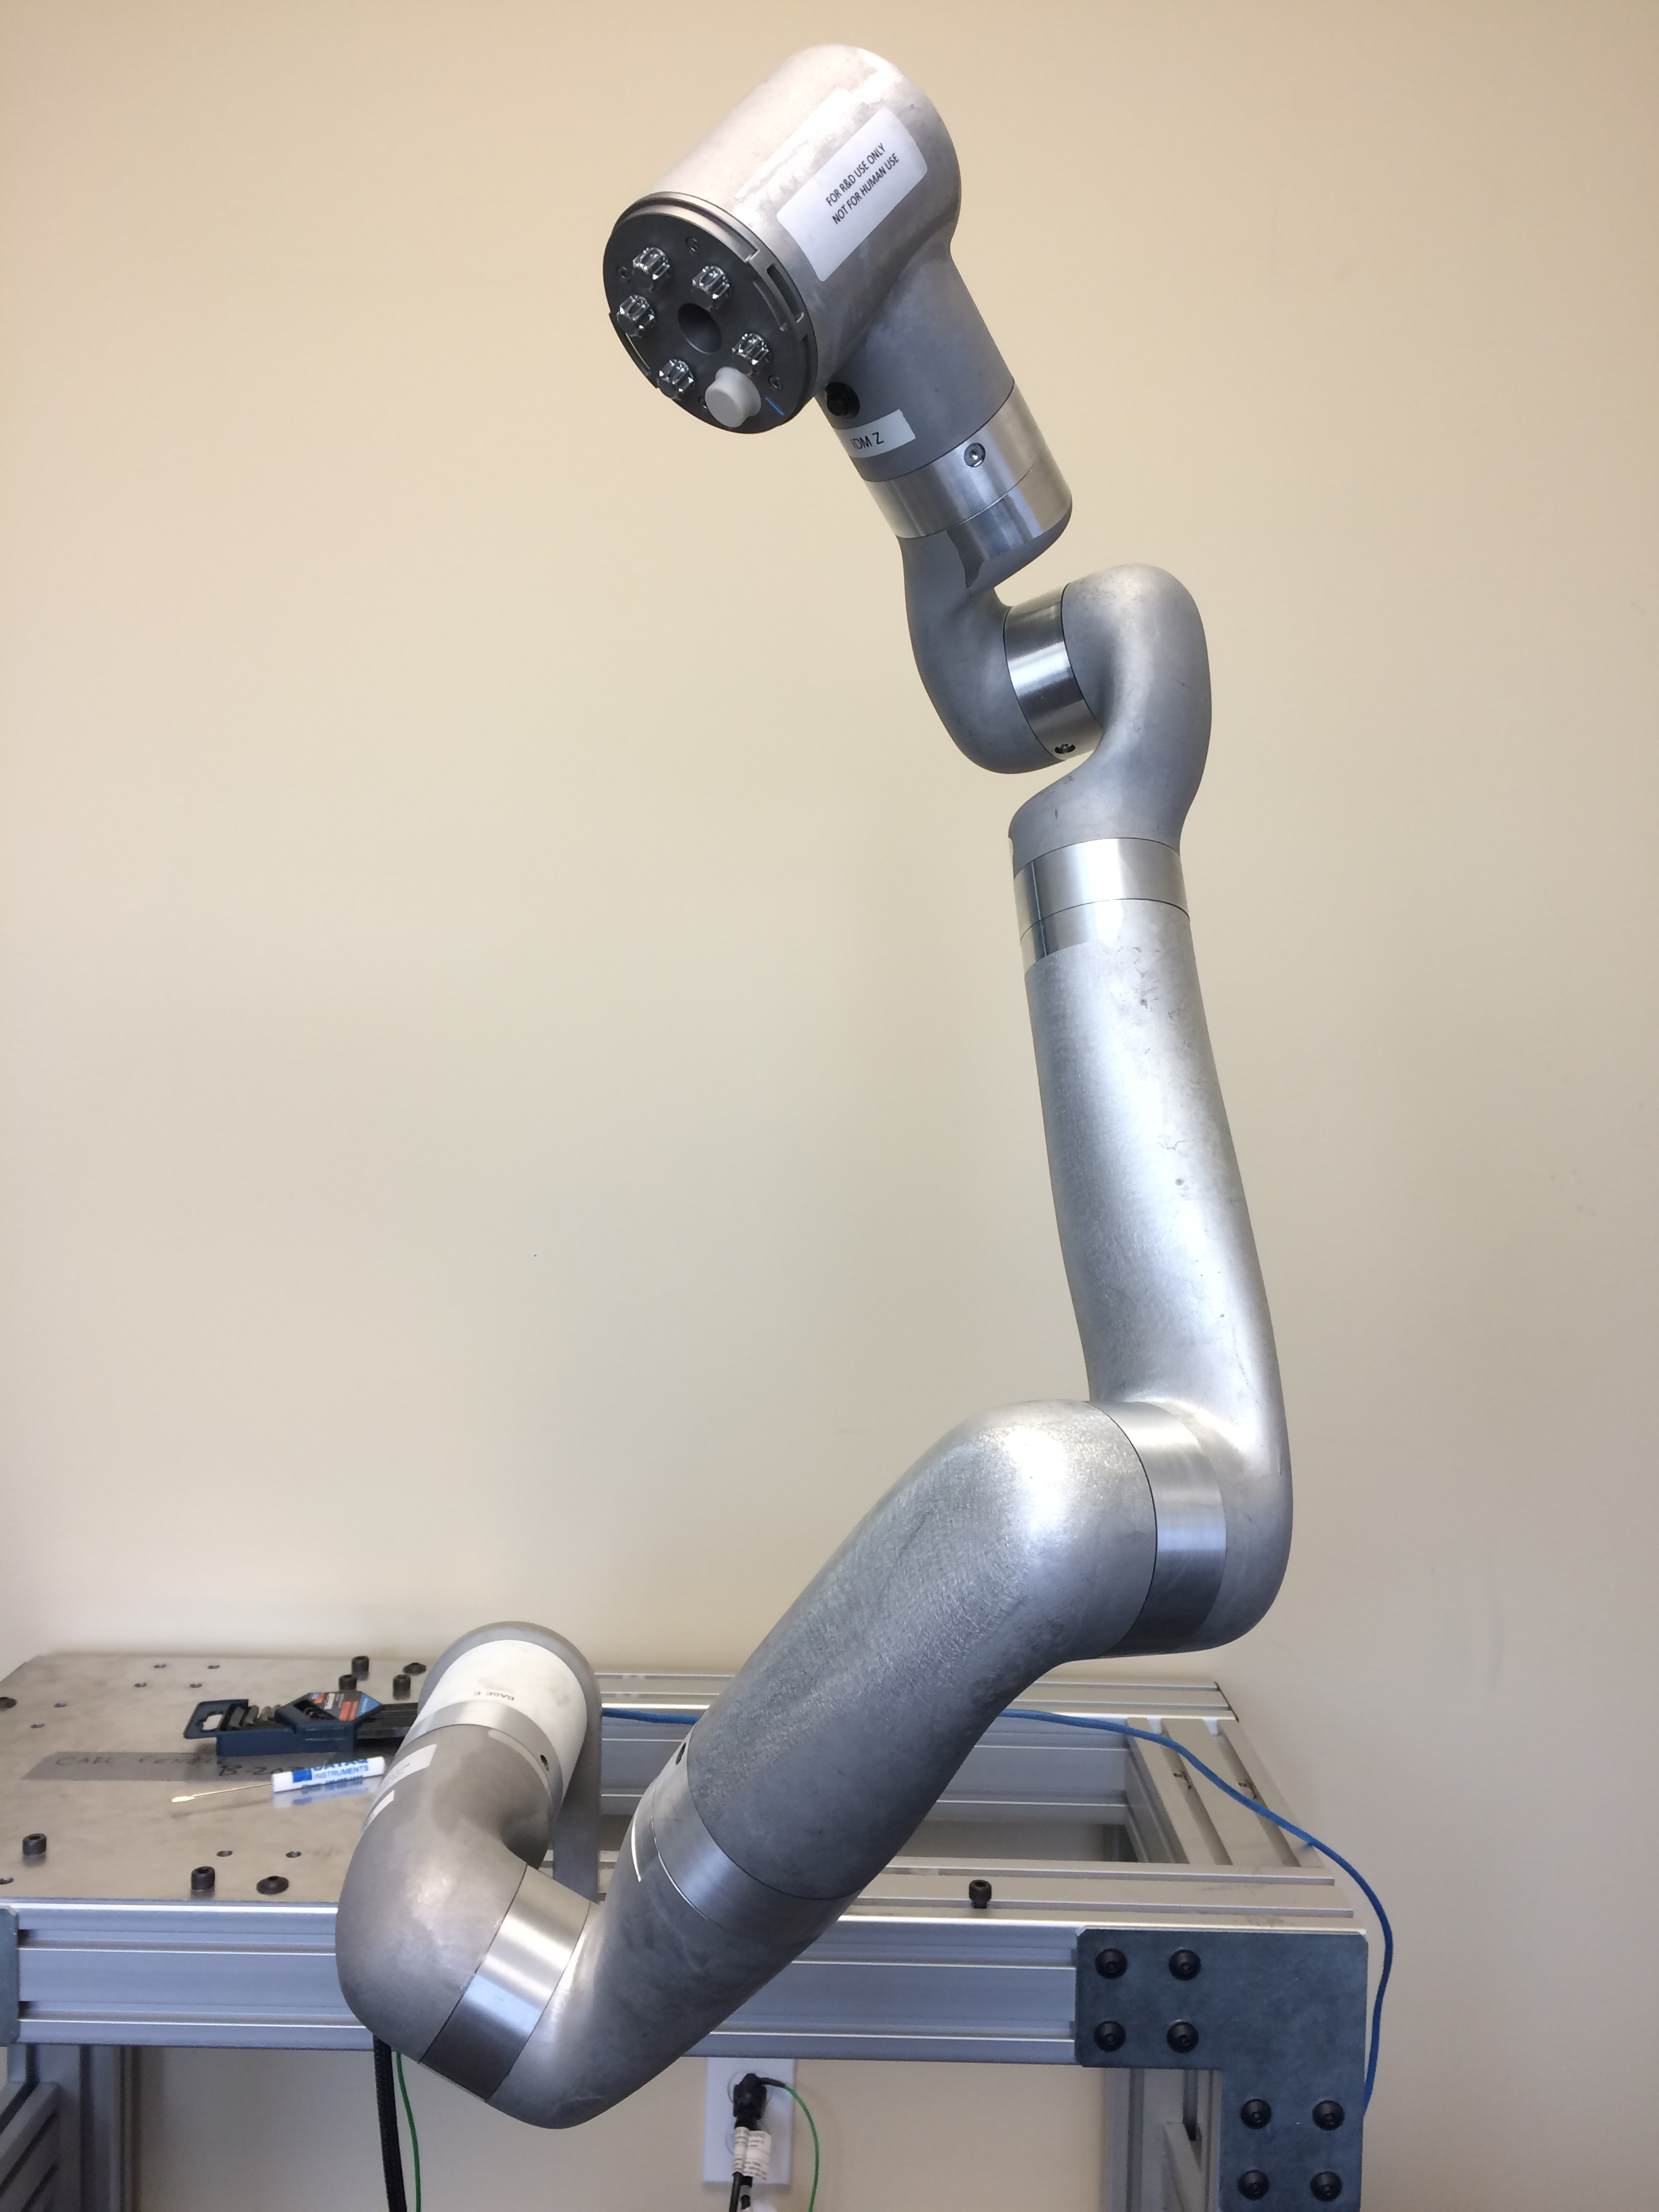
\includegraphics[width=0.9\textwidth]{./images/Pose7}
		\captionof{figure}{Pose7}
		\label{fig:pose7}
	\end{minipage}%
	\begin{minipage}{.5\textwidth}
		\centering
		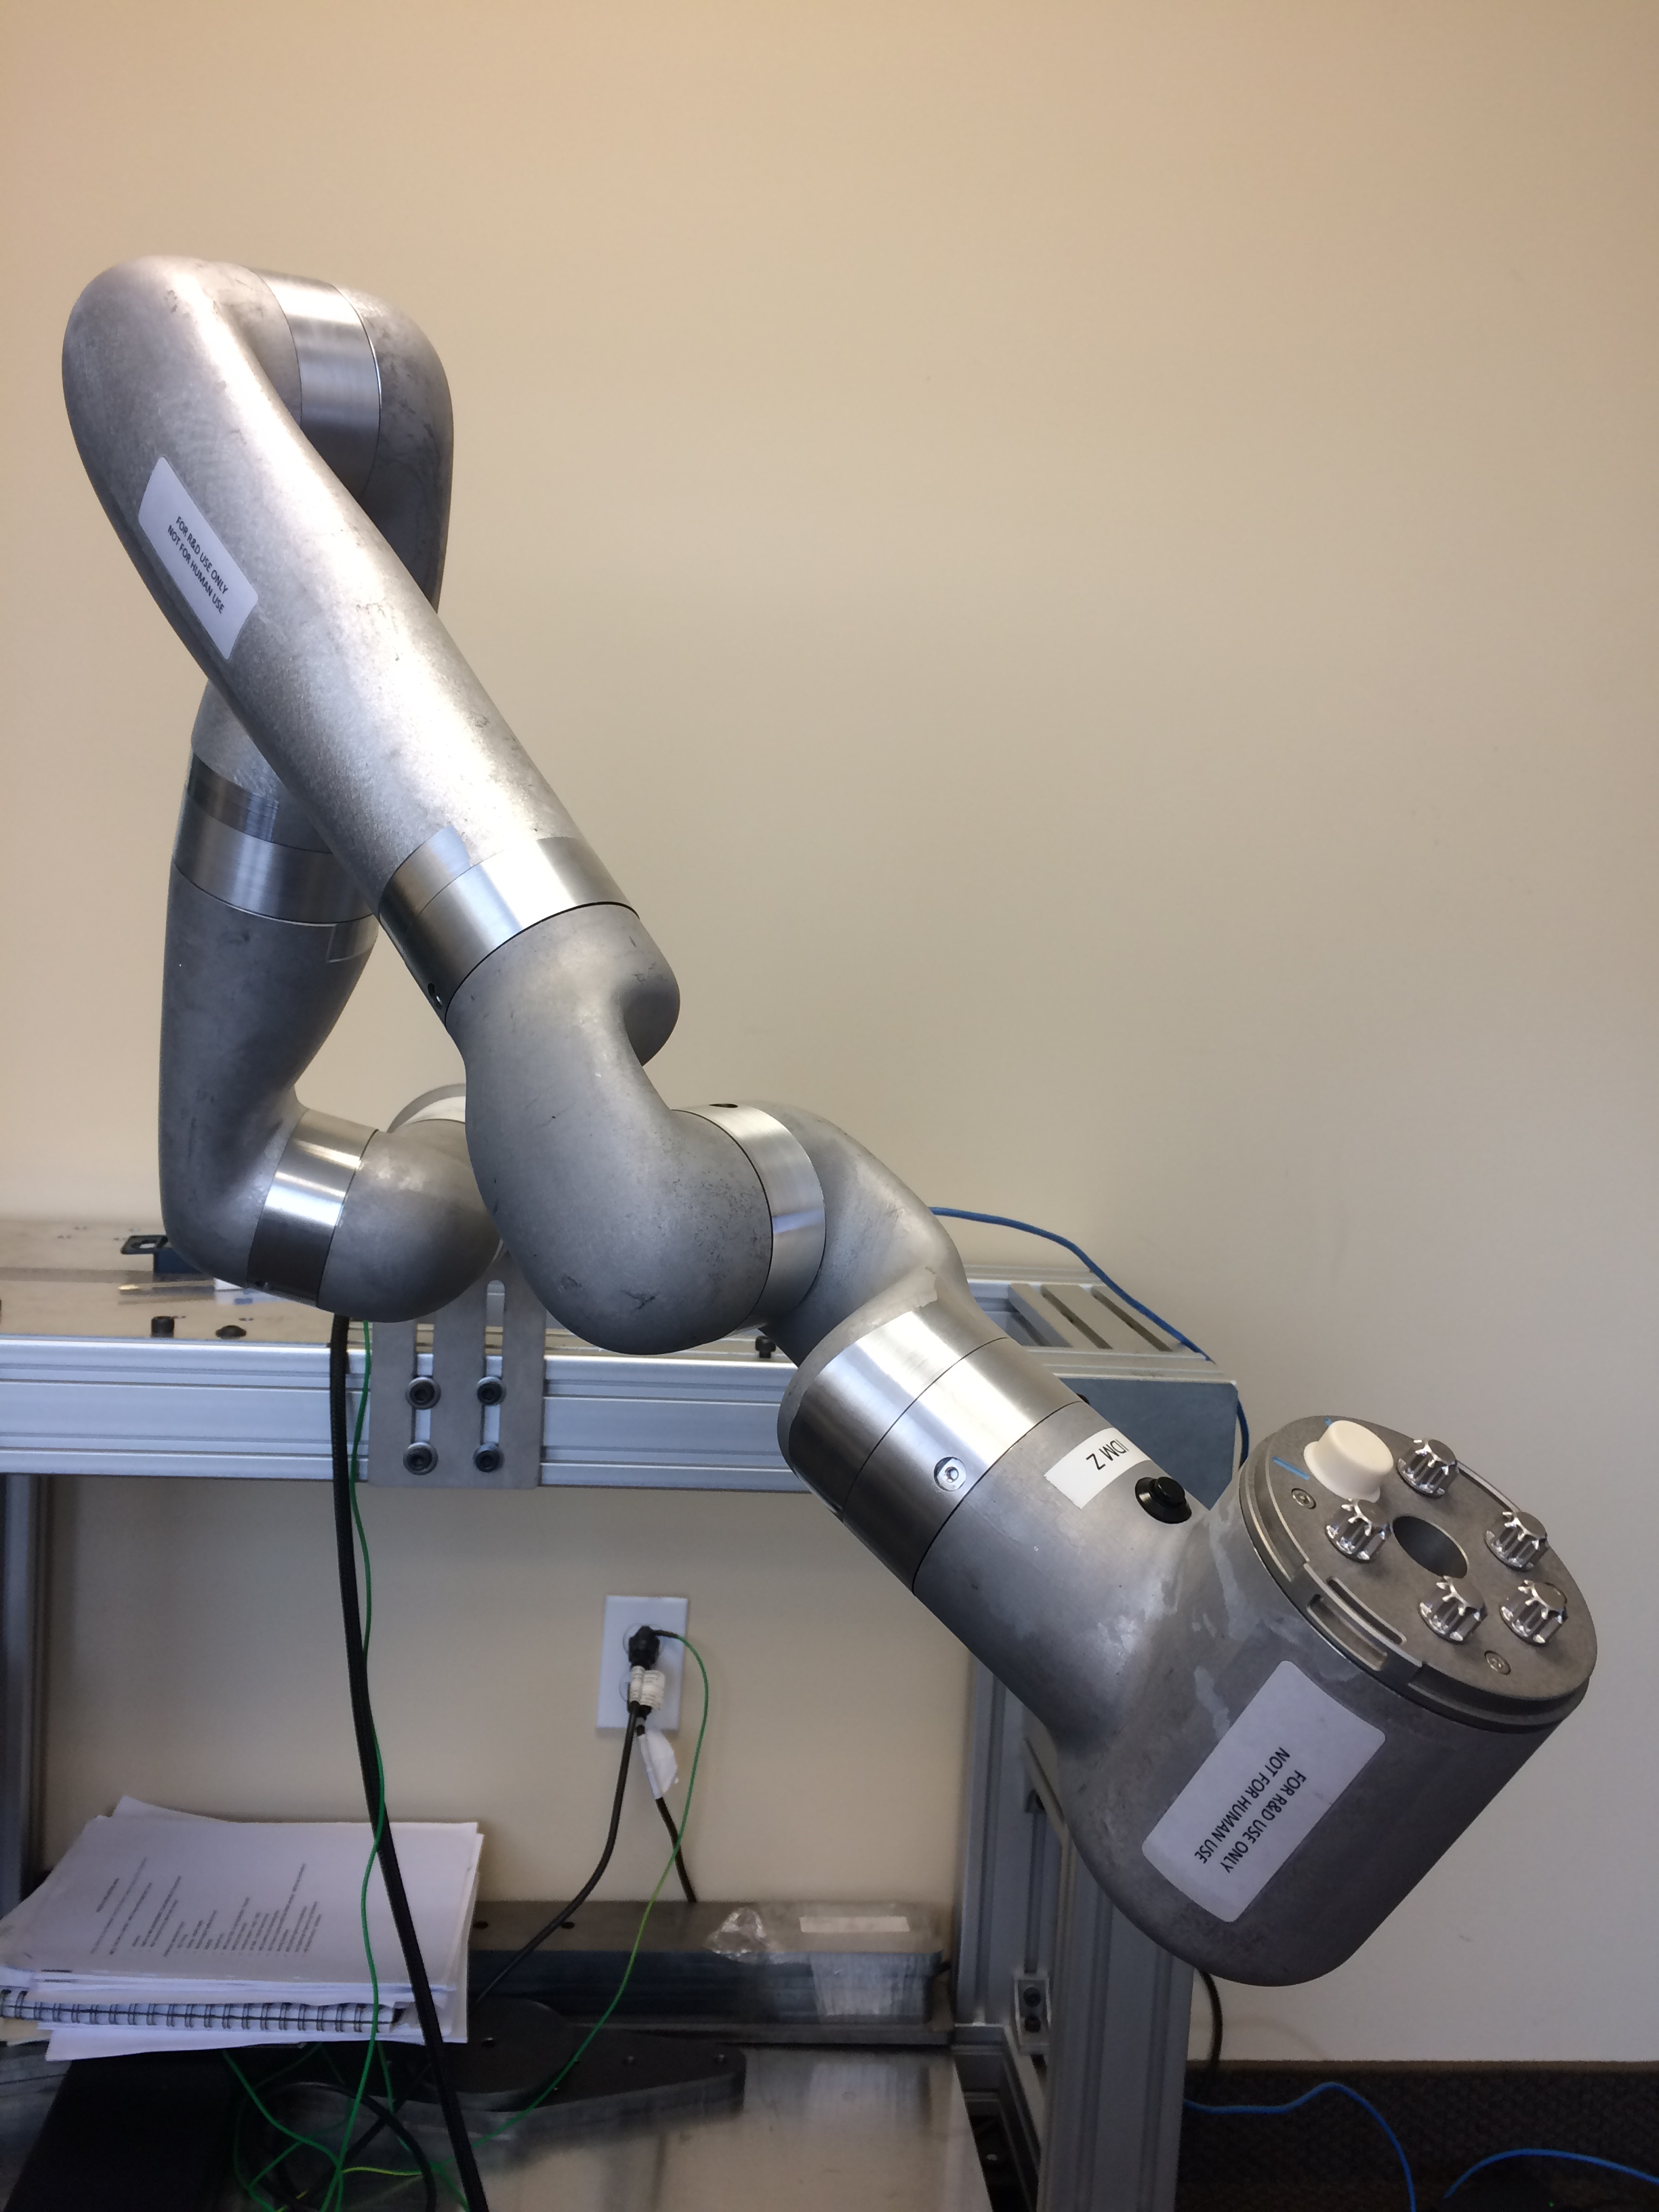
\includegraphics[width=0.9\textwidth]{./images/Pose8}
		\captionof{figure}{Pose8}
		\label{fig:pose8}
	\end{minipage}
\end{figure}

\begin{figure}
	\centering
	\begin{minipage}{.5\textwidth}
		\centering
		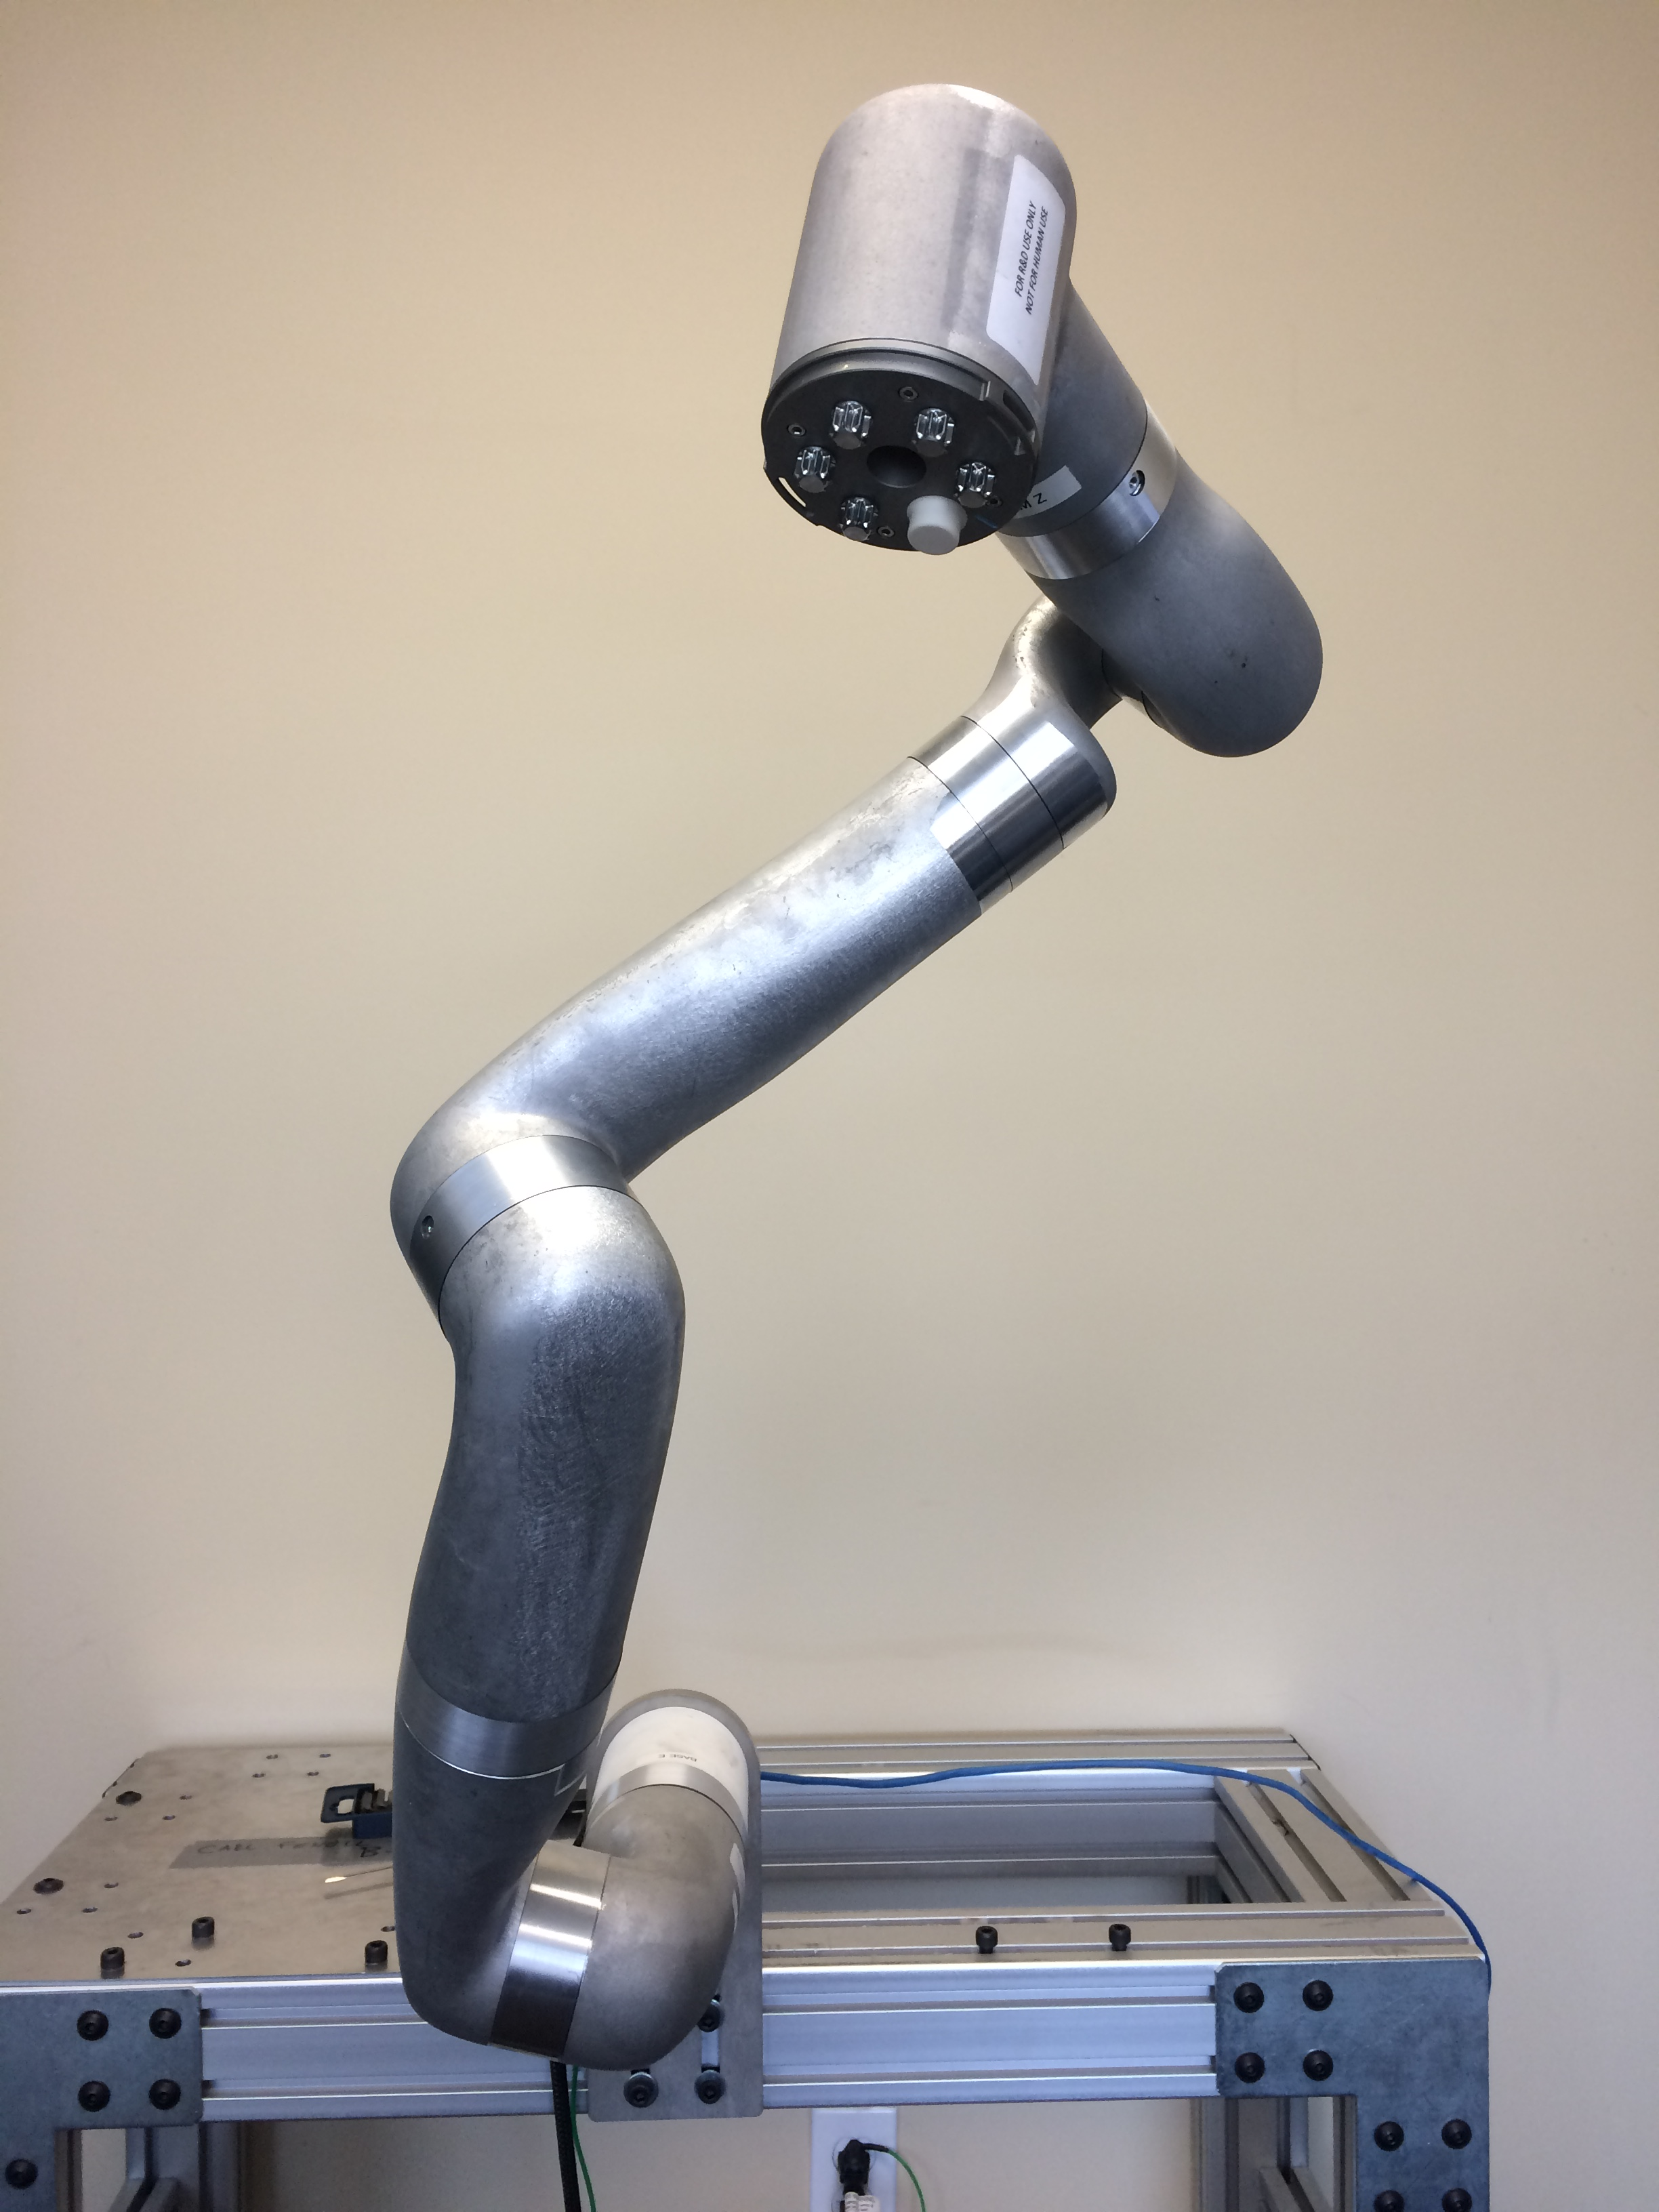
\includegraphics[width=0.9\textwidth]{./images/Pose9}
		\captionof{figure}{Pose9}
		\label{fig:pose9}
	\end{minipage}%
	\begin{minipage}{.5\textwidth}
		\centering
		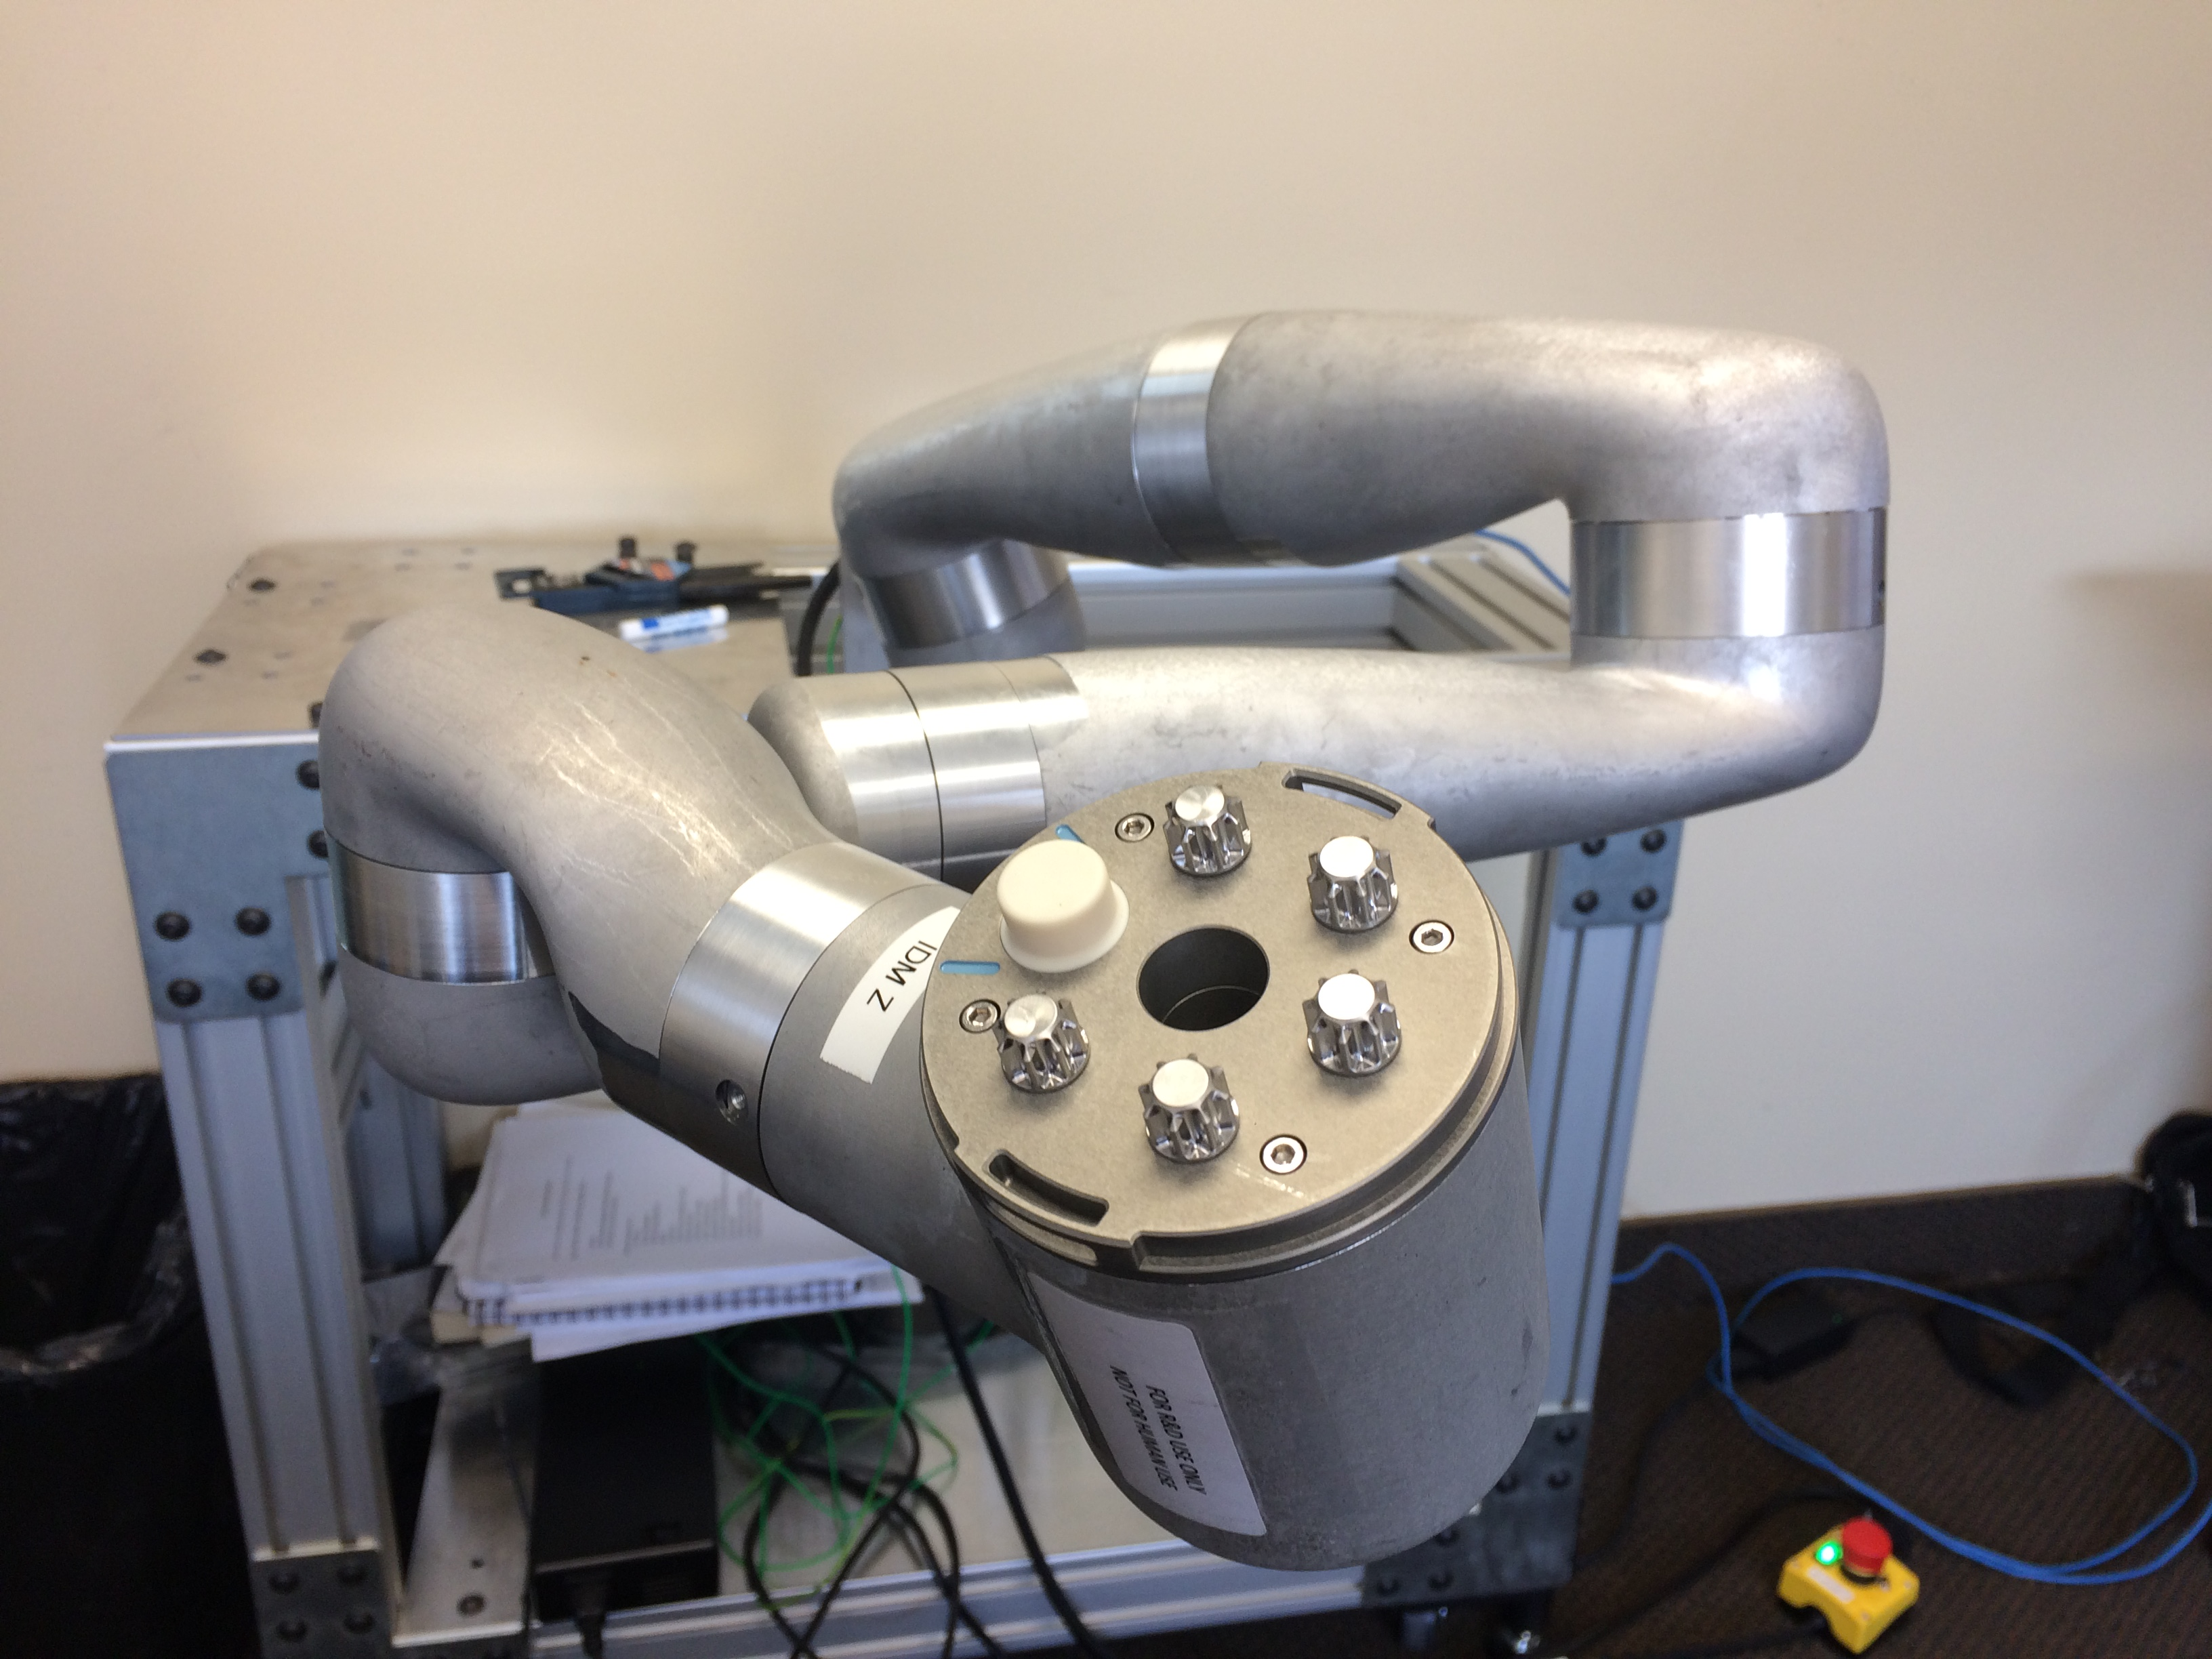
\includegraphics[width=0.9\textwidth]{./images/Pose10}
		\captionof{figure}{Pose10}
		\label{fig:pose10}
	\end{minipage}
\end{figure}



\textbf{Group B}
In the second group (see in Table \ref{table-groupB}), the robot configurations are defined to have a maximum load on one or several joints. Since there is no extra load on the robot end-effector, the load only takes robot arm and IDM into account. 


\begin{table}[]
	\centering
	\caption{Pre-defined Robot Configuration of Group B (Degrees)}
	\label{table-groupB}
	\begin{tabular}{|l|r|r|r|r|r|r|r|r|}
		\hline
		\textbf{}  & \textbf{Joint1} & \textbf{Joint2} & \textbf{Joint3} & \textbf{Joint4} & \textbf{Joint5} & \textbf{Joint6} & \textbf{Joint7} & \textbf{Maximum Load} \\ \hline
		\textbf{Pose 11} & 180   & 180   & 180    & 180   & 180   & 180   & 180   & No load to all (Figure \ref{fig:pose11})   \\ \hline
		\textbf{Pose 12} & 270   & 180   & 180    & 180   & 180   & 180   & 180   & Joint 2, 4, 6, 7 (Figure \ref{fig:pose12}) \\ \hline
		\textbf{Pose 13} & 180   & 180   & 180    & 180   & 180   & 90   & 180   & Joint 5 (Figure \ref{fig:pose13})      \\ \hline
		\textbf{Pose 14} & 180   & 180   & 180    & 90   & 180   & 180   & 180   & Joint 3 (Figure \ref{fig:pose14})      \\ \hline
		\textbf{Pose 15} & 180   & 90   & 180    & 180   & 180   & 180   & 180   & Joint 1 (Figure \ref{fig:pose15})      \\ \hline
	\end{tabular}
\end{table}


\begin{figure}
	\centering
	\begin{minipage}{.5\textwidth}
		\centering
		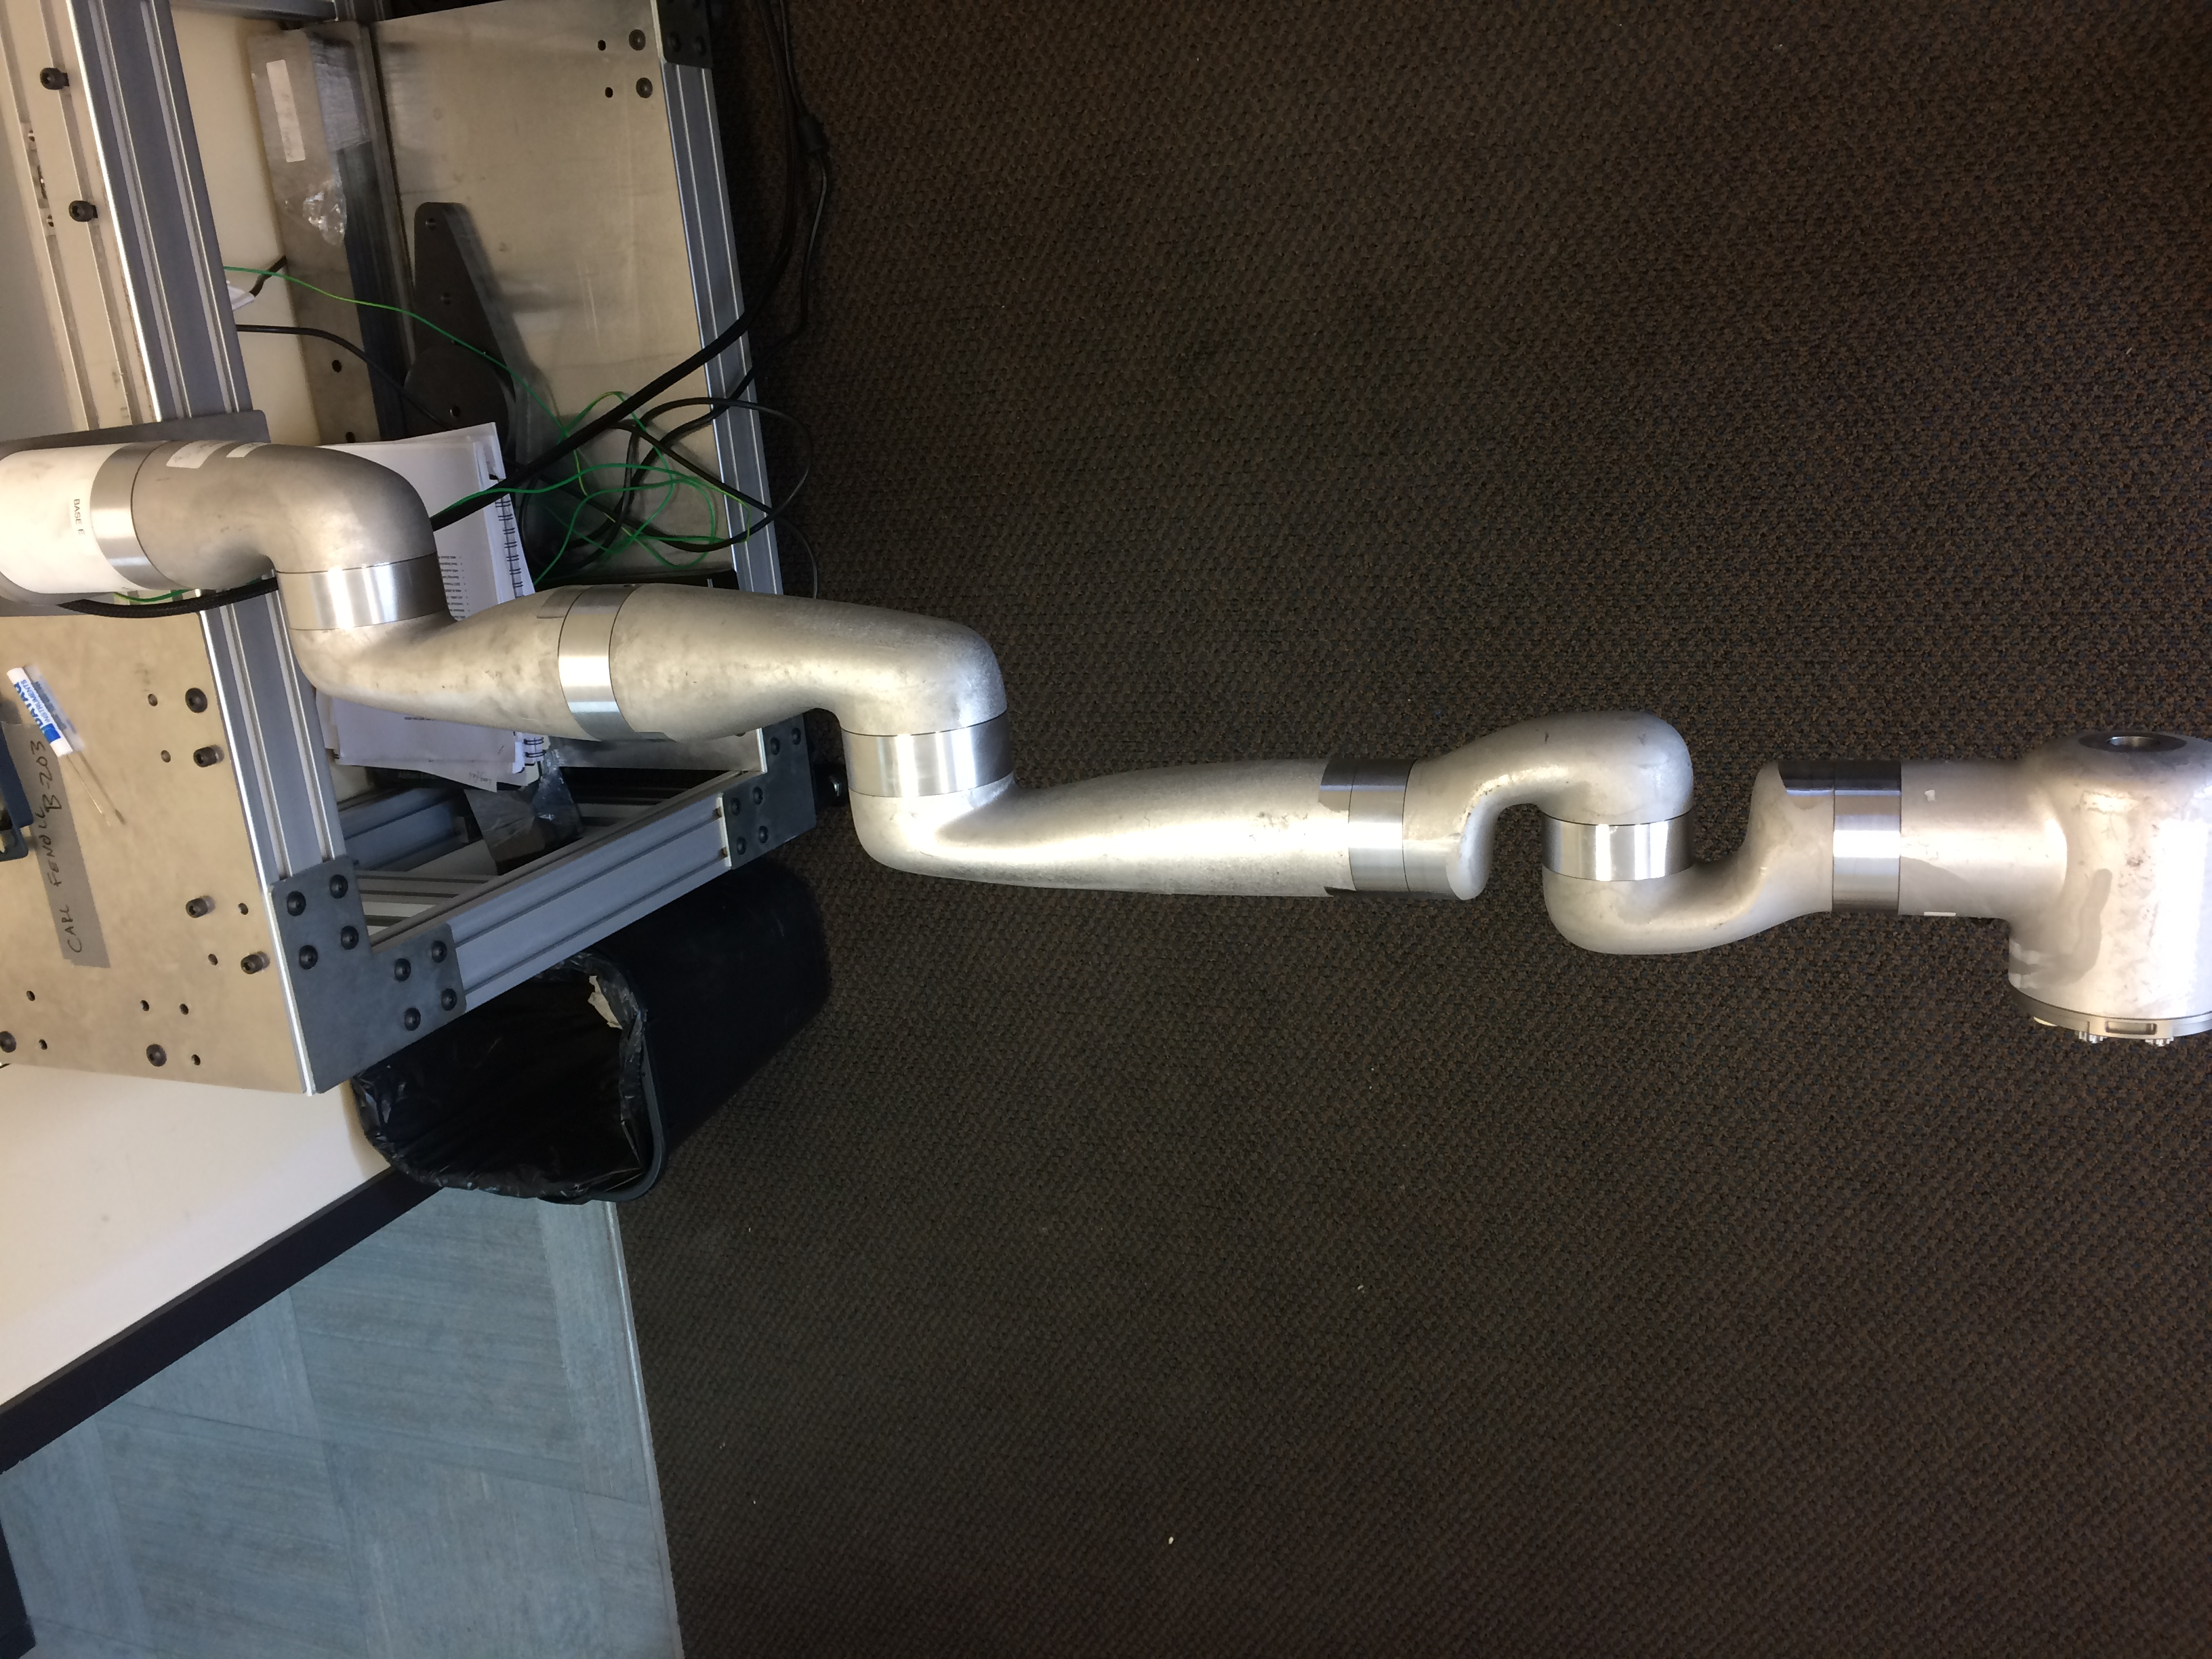
\includegraphics[width=0.9\textwidth]{./images/Pose12}
		\captionof{figure}{Pose12}
		\label{fig:pose12}
	\end{minipage}%
	\begin{minipage}{.5\textwidth}
		\centering
		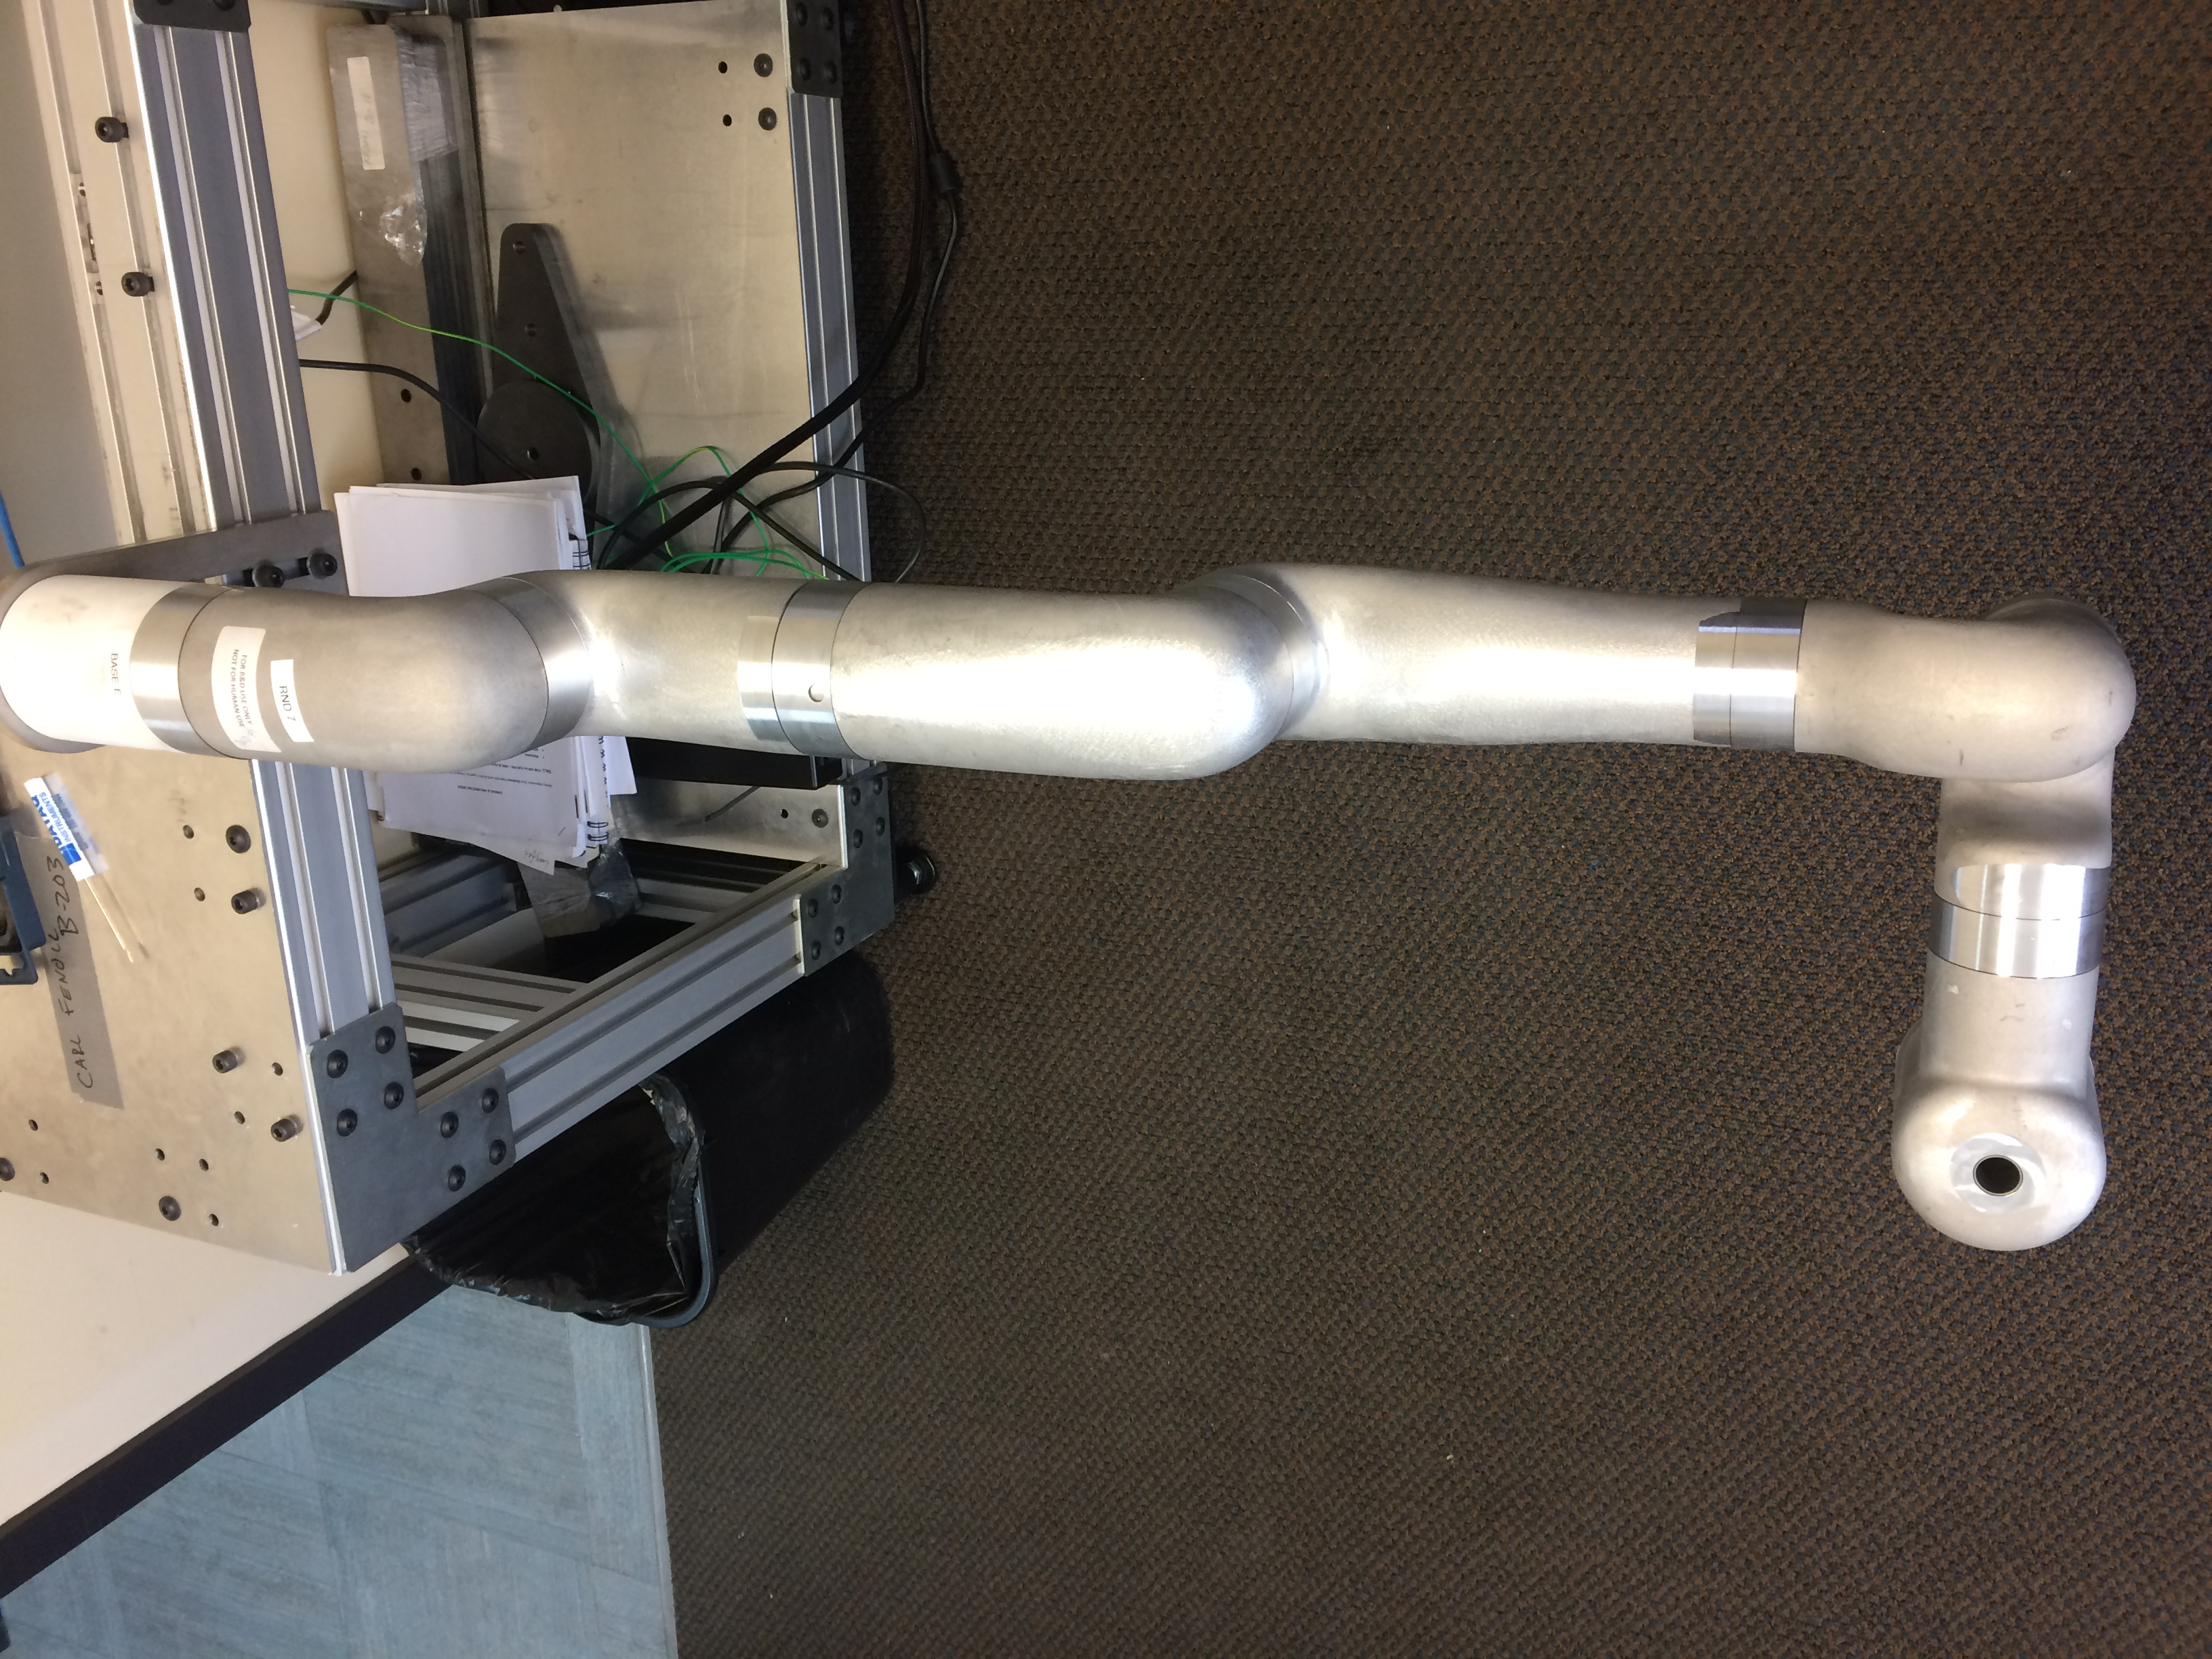
\includegraphics[width=0.9\textwidth]{./images/Pose13}
		\captionof{figure}{Pose13}
		\label{fig:pose13}
	\end{minipage}
\end{figure}

\begin{figure}
	\centering
	\begin{minipage}{.5\textwidth}
		\centering
		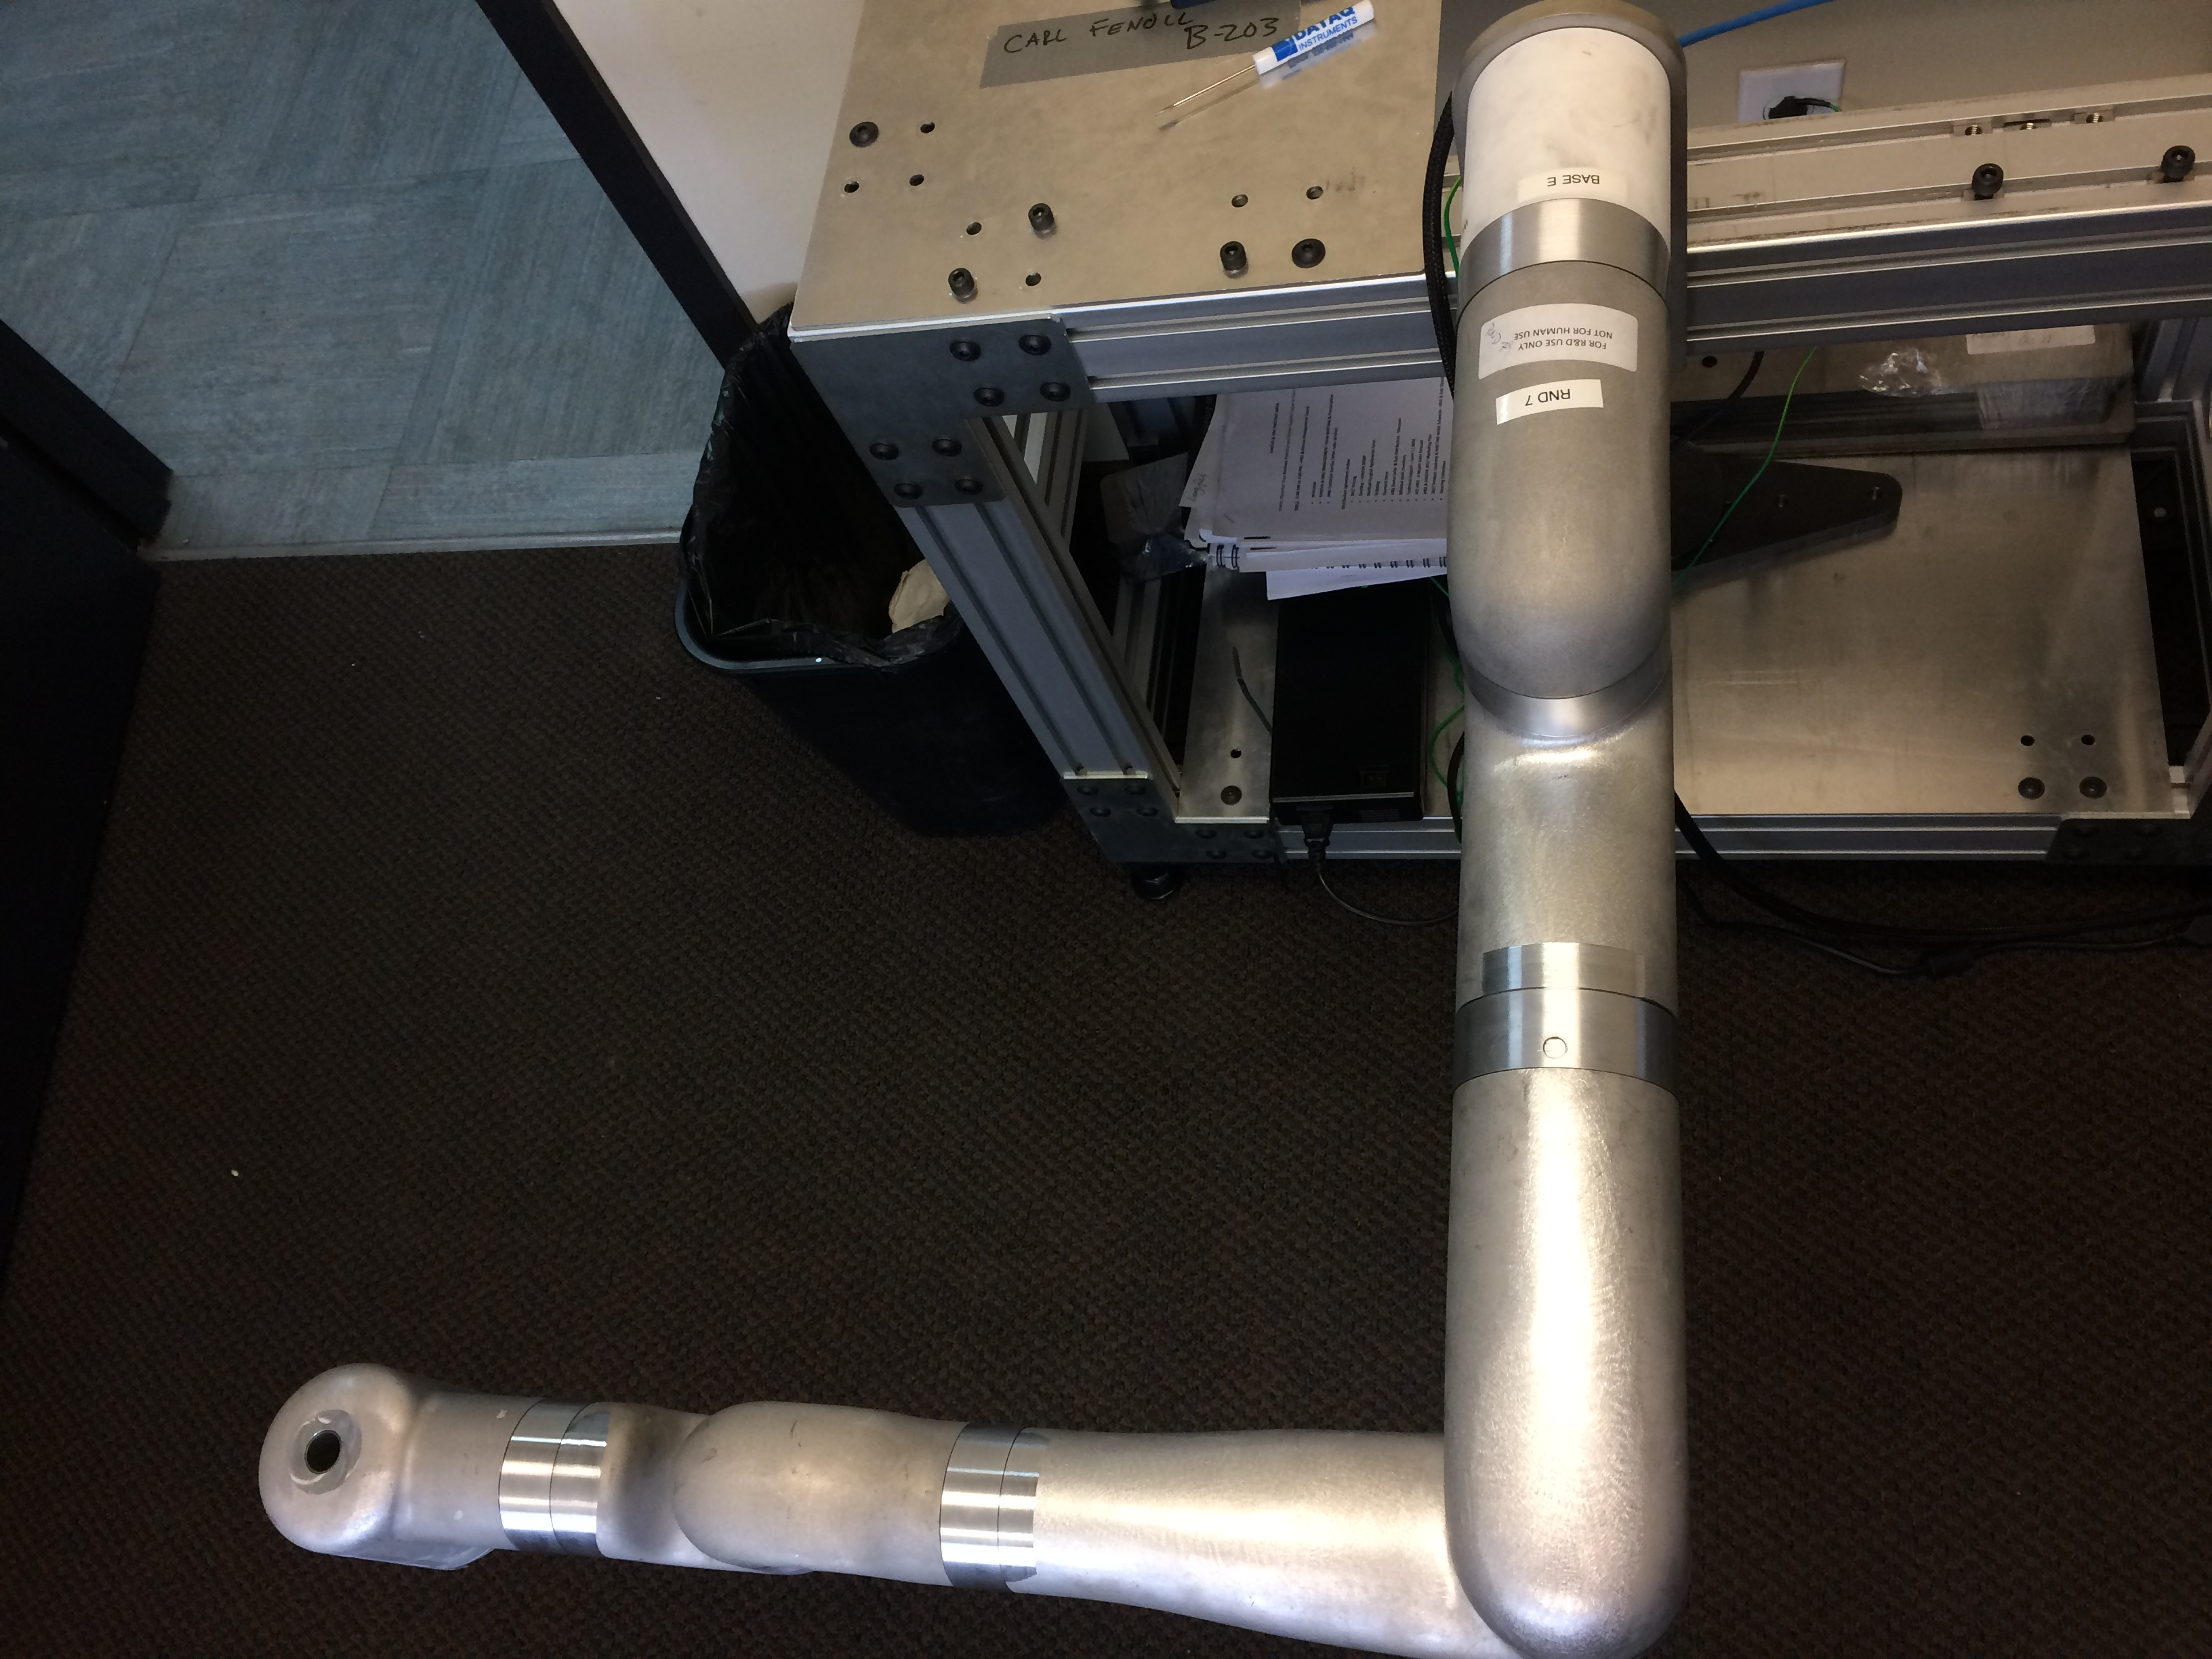
\includegraphics[width=0.9\textwidth]{./images/Pose14}
		\captionof{figure}{Pose14}
		\label{fig:pose14}
	\end{minipage}%
	\begin{minipage}{.5\textwidth}
		\centering
		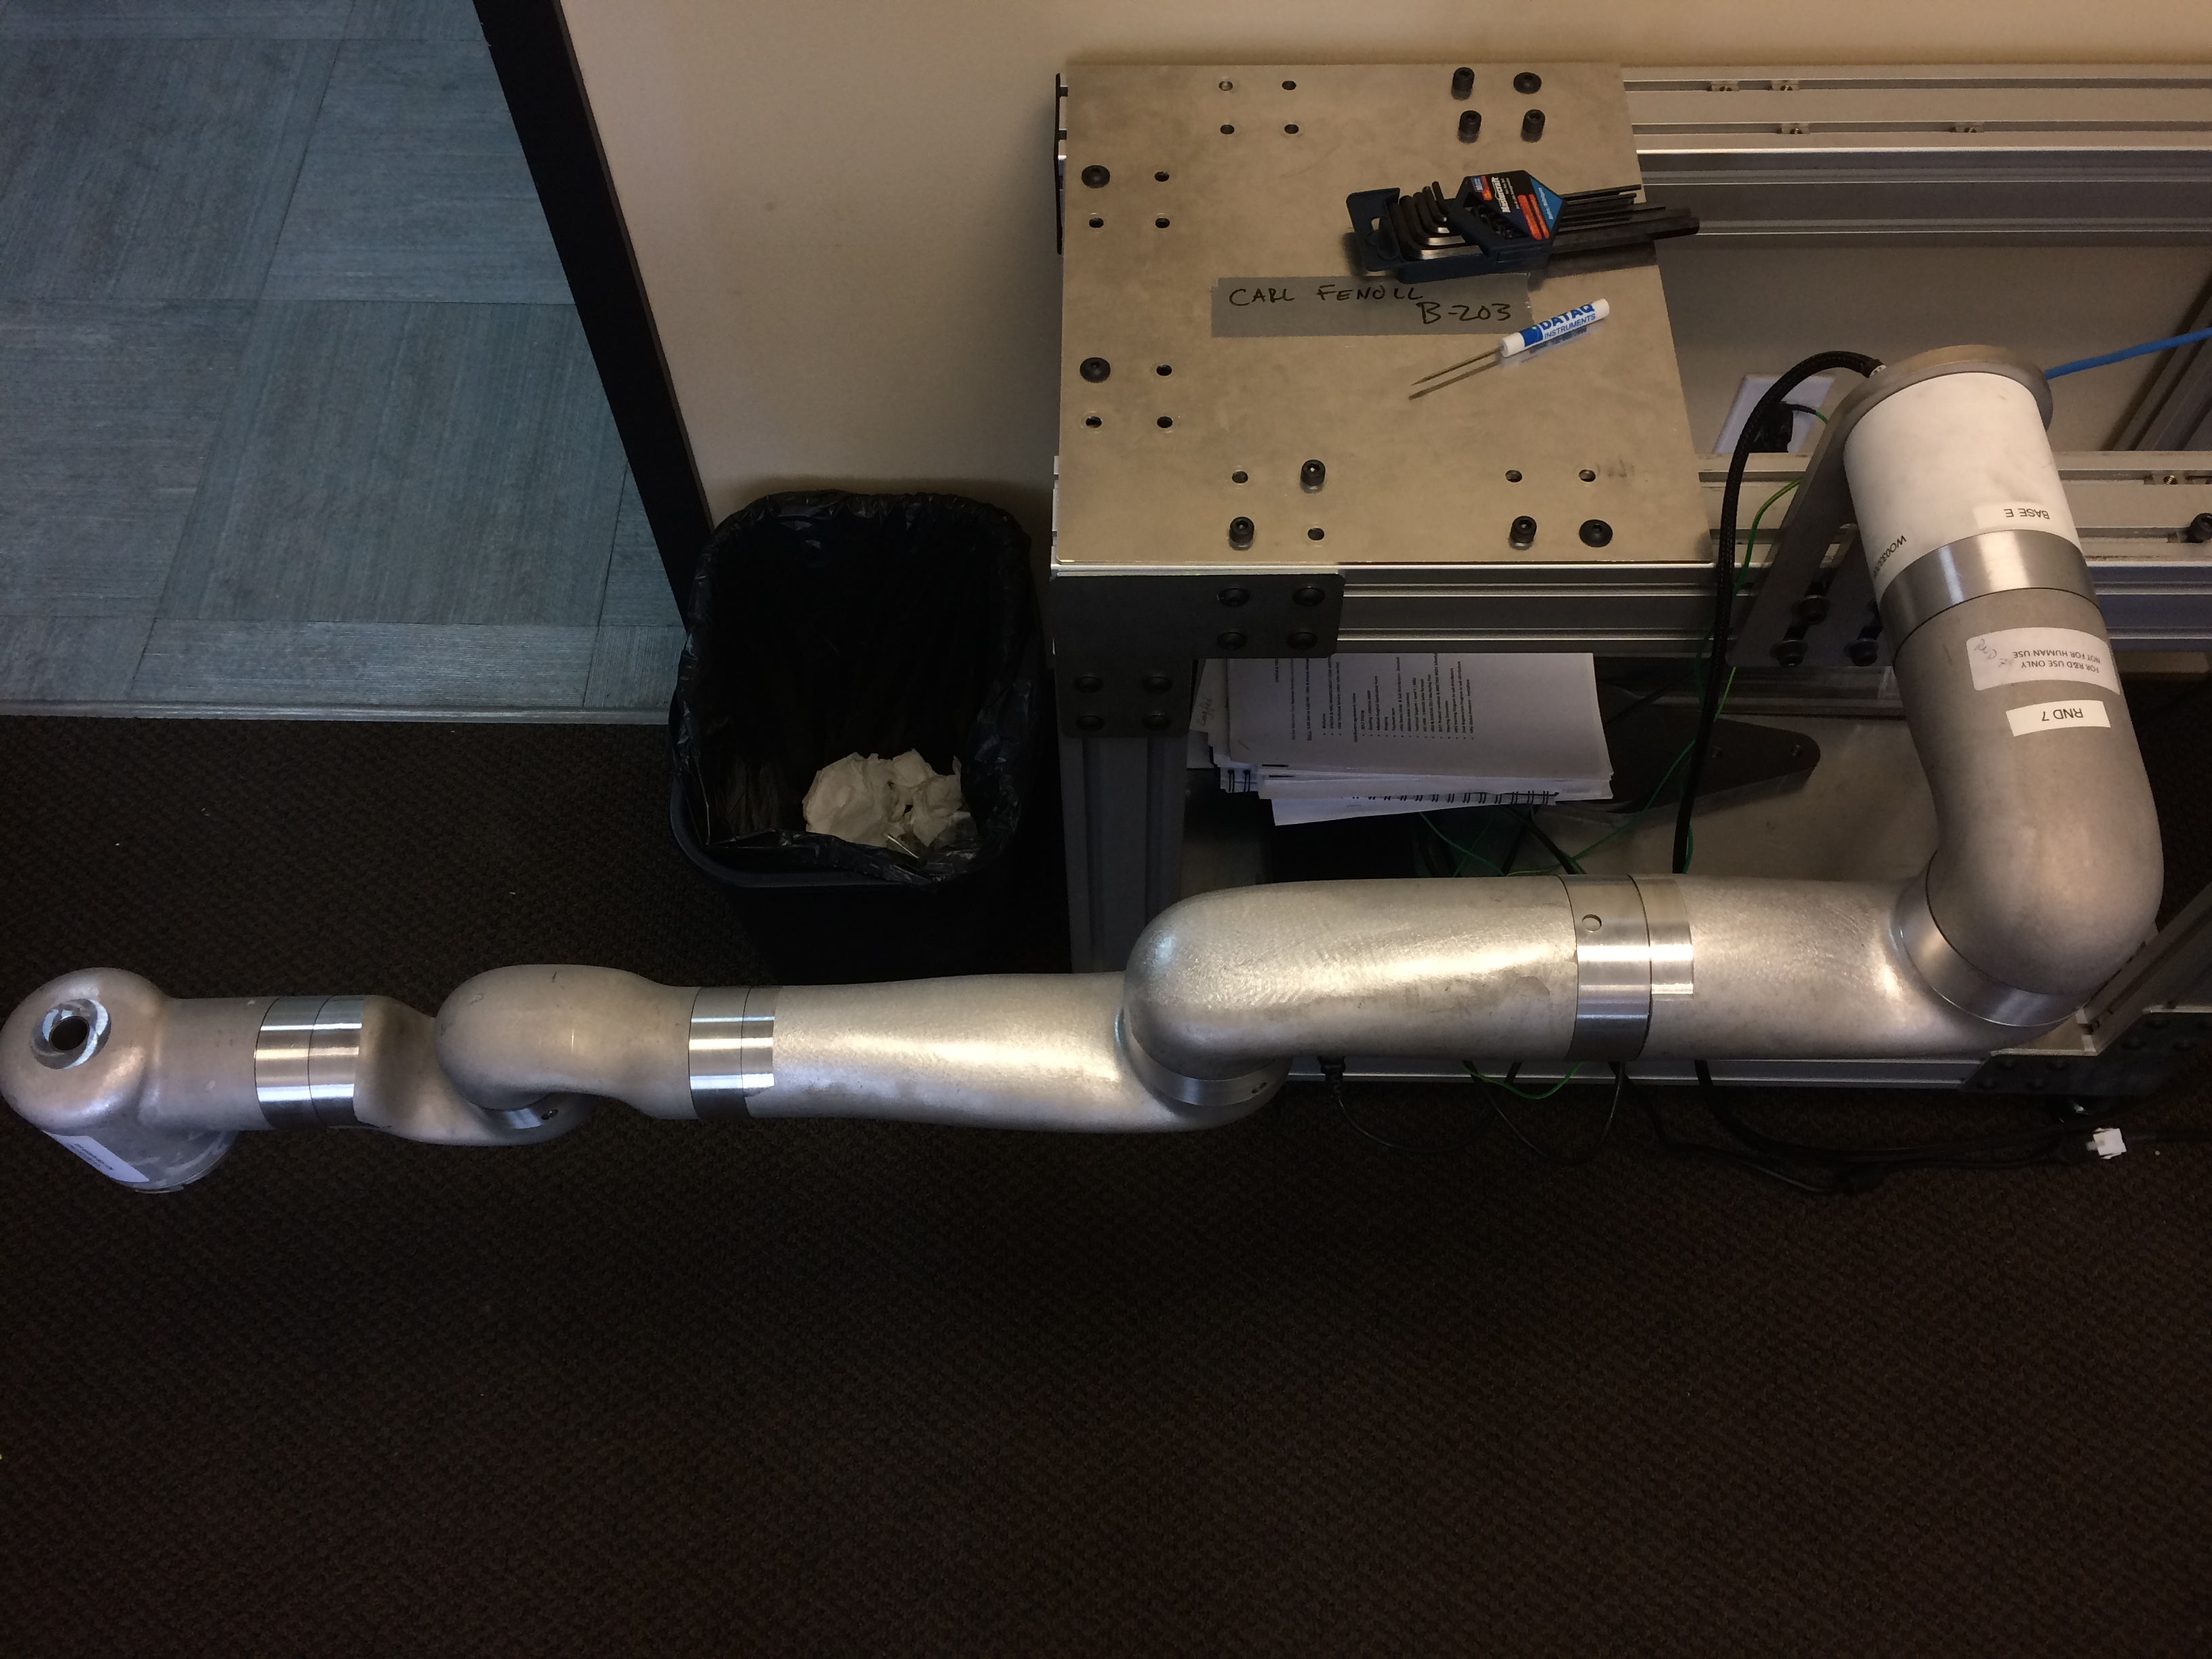
\includegraphics[width=0.9\textwidth]{./images/Pose15}
		\captionof{figure}{Pose15}
		\label{fig:pose15}
	\end{minipage}
\end{figure}



